
\chapter{立体積層フレームの製作工程について}
立体フレームを成型するための型は,3DCADにて設計を行い3Dプリンターを用いて制作を行った.

\begin{figure}[htbp]
  \begin{center}
    \includegraphics[width=120mm]{img/6.JPG}
    \end{center}
  \caption{立体フレームの3Dモデル}
 \label{fig:robot}
\end{figure}

\section{プリンターでの立体型造形}
3Dプリンターでの造形には,各型につきそれぞれ6時間から7時間を要した.立体型は雄型,雌型をそれぞれの設計を行った.平面用の木枠は一体型に対し,立体フレーム用の型は大きさの関係上,造形時のプリンターのテーブルに収まらないため二つのパーツに分けて設計をした.積層時に連結するための突起部分も設計されている.また,造形時プリンターのノズルからの樹脂の射出温度と空冷時の室内温度の温度差が大きくなってしまう場合があった.その結果,反りが発生してしまい造形途中でクラックが入ったり,土台がテーブルから浮いてしまうなど,全体のゆがみの原因となってしまった.そのための土台の表面積を増加させ,テーブルにはのりを付着させそれらの防止をする工夫を施した.

\begin{figure}[htbp]
  \begin{center}
    \includegraphics[width=120mm]{img/8.JPG}
    \end{center}
  \caption{造形された型}
 \label{fig:robot}
\end{figure}

\begin{figure}[htbp]
  \begin{center}
    \includegraphics[width=120mm]{img/9.JPG}
    \end{center}
  \caption{型の連結部分}
 \label{fig:robot}
\end{figure}

\section{立体型への離型剤塗り付け作業}
立体フレーム用の型には離型剤として,車用のワックスを利用した.むらができてしまうと離型が困難になってしまうため,ワックスは厚めにぬりこんだ.また圧縮用のポリ袋にはくっつかず容易に離型することができる.

\begin{figure}[htbp]
  \begin{center}
    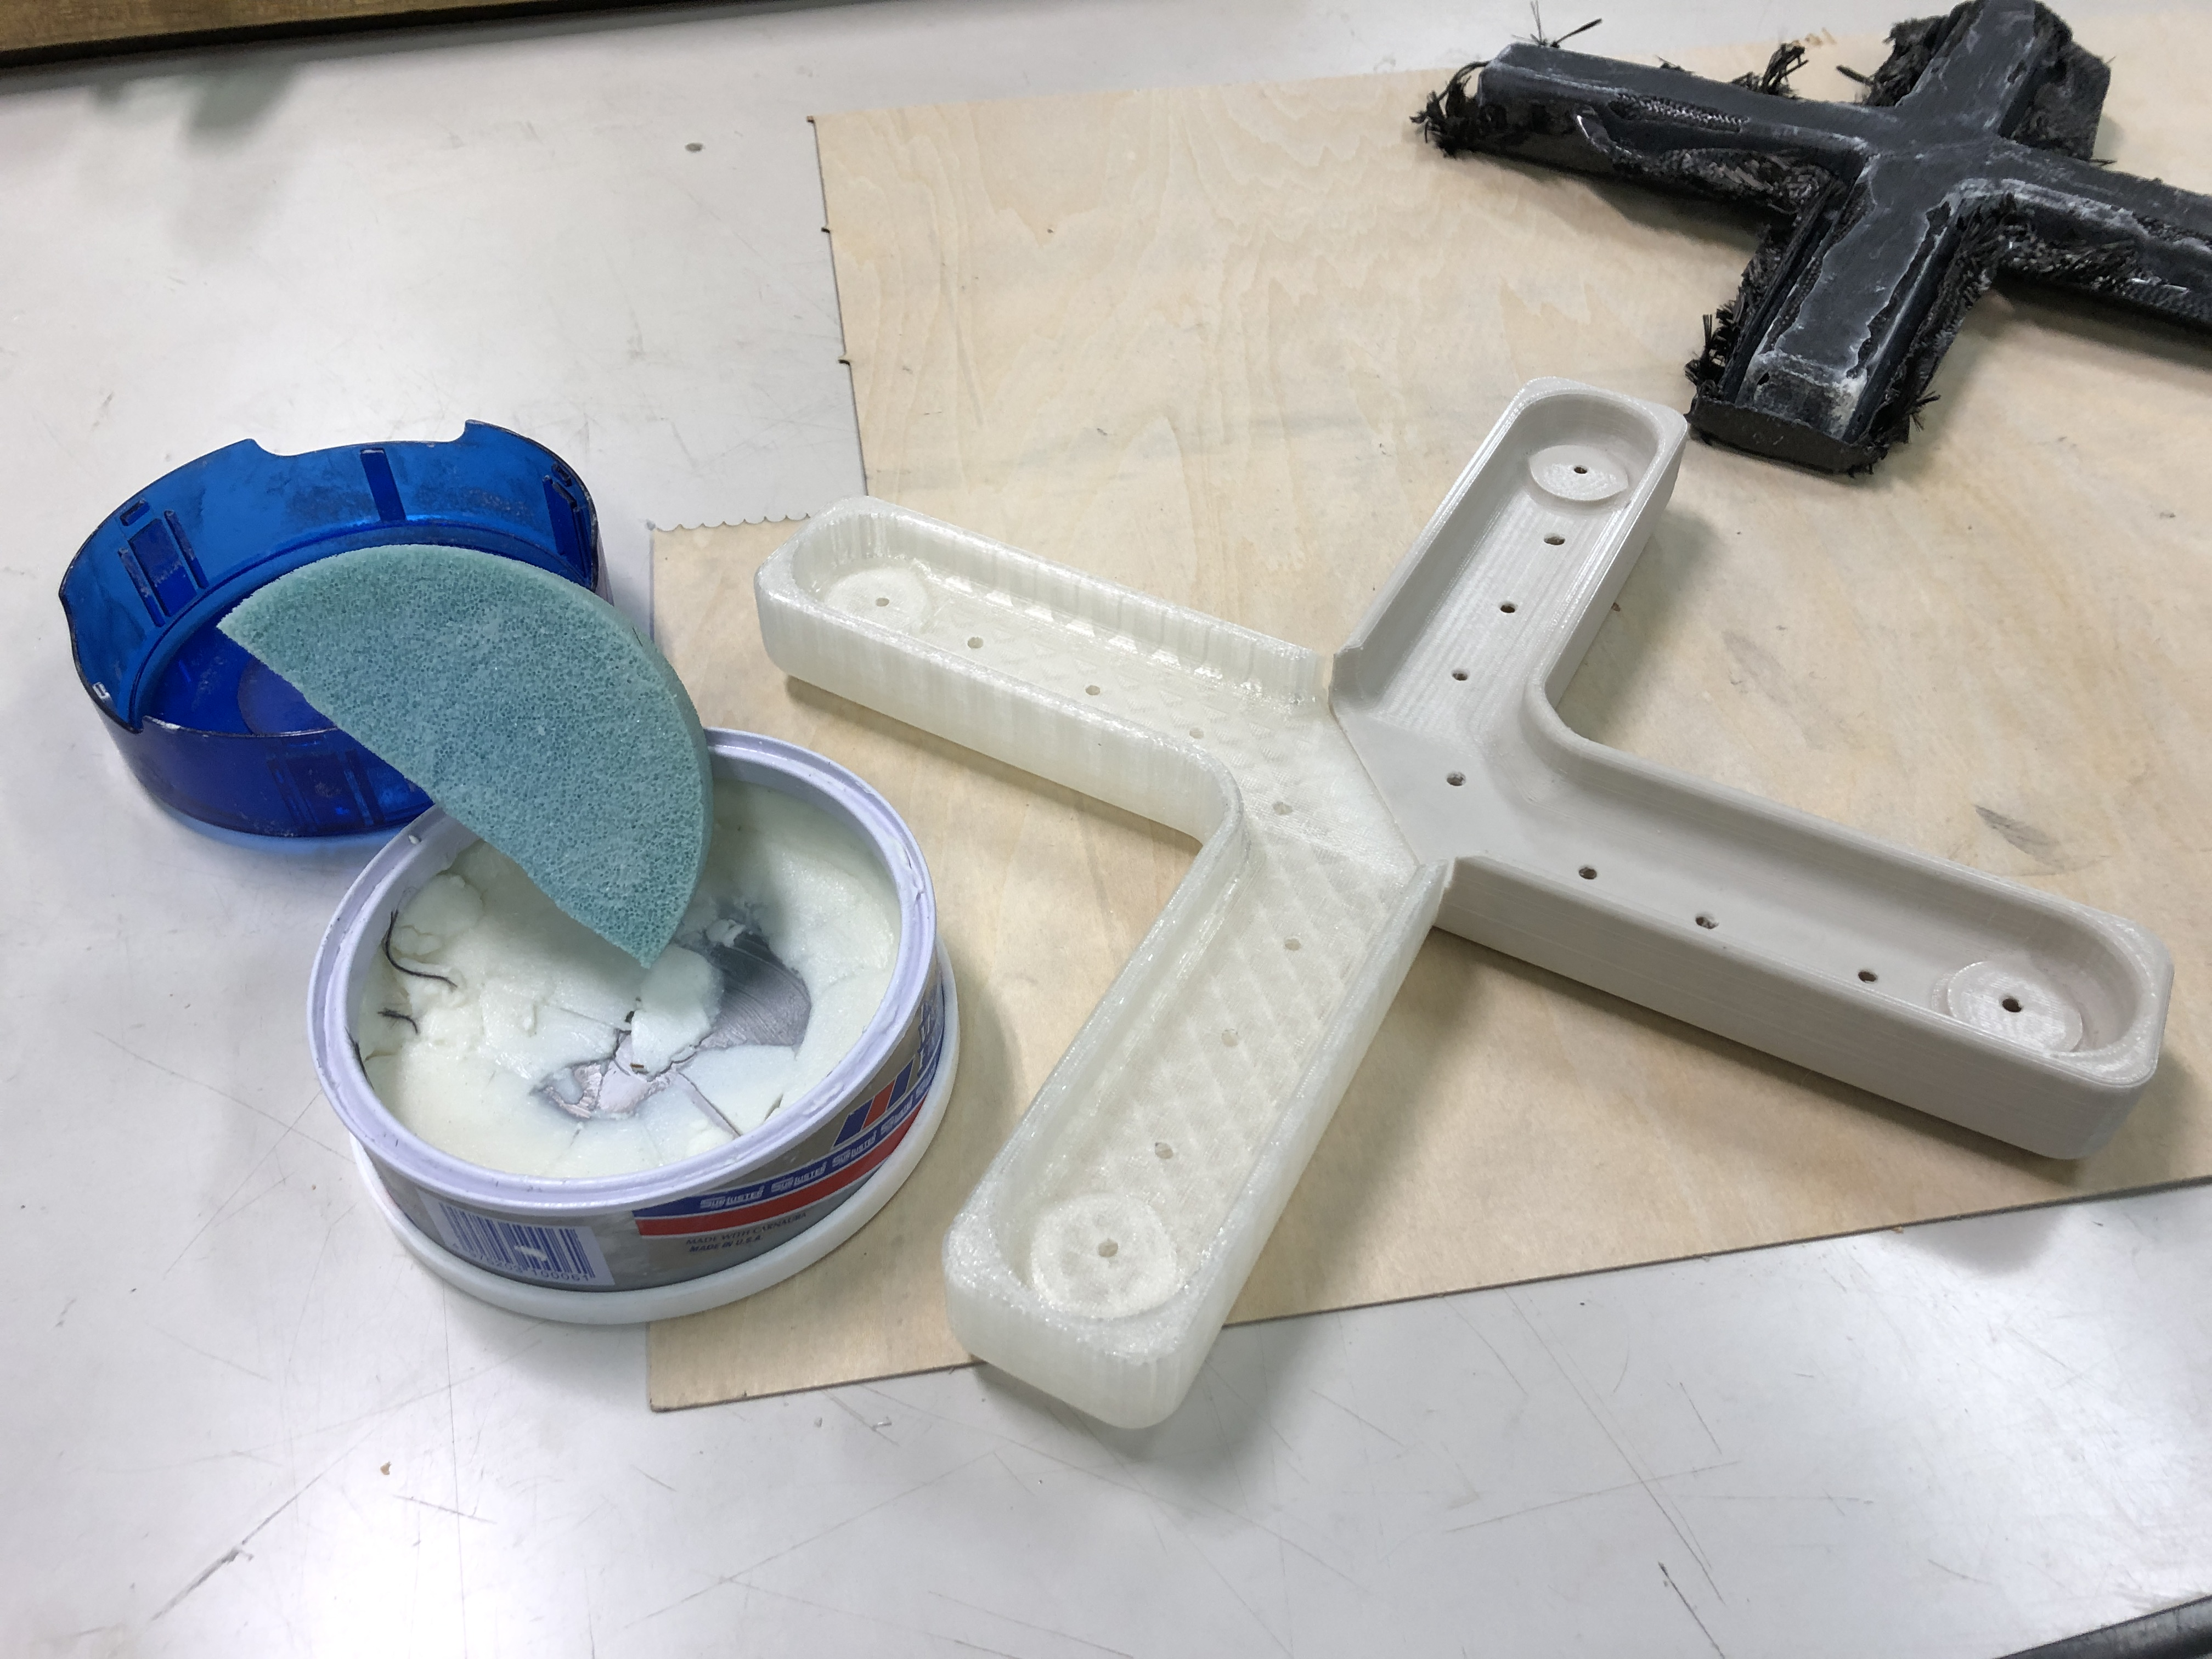
\includegraphics[width=120mm]{img/10.JPG}
    \end{center}
  \caption{ワックスの塗り付け}
 \label{fig:robot}
\end{figure}



\section{積層作業}
離型剤を塗った型にカーボンシートを被せ積層を行っていく.この際に一枚をフレームの形に多い壁せていくのはしわができてしまったりと困難なため,四分割にして行った.型内部の縁に沿って折り目をつけていき,エポキシ樹脂を刷毛で塗っていく.二枚目以降も同様に積層作業を行い,隙間やエッジ部分のしわを極力少なくしてゆく.またカーボンシート枚数を重ねるごとにエポキシ樹脂の量を減少させていく.

\begin{figure}[htbp]
  \begin{center}
    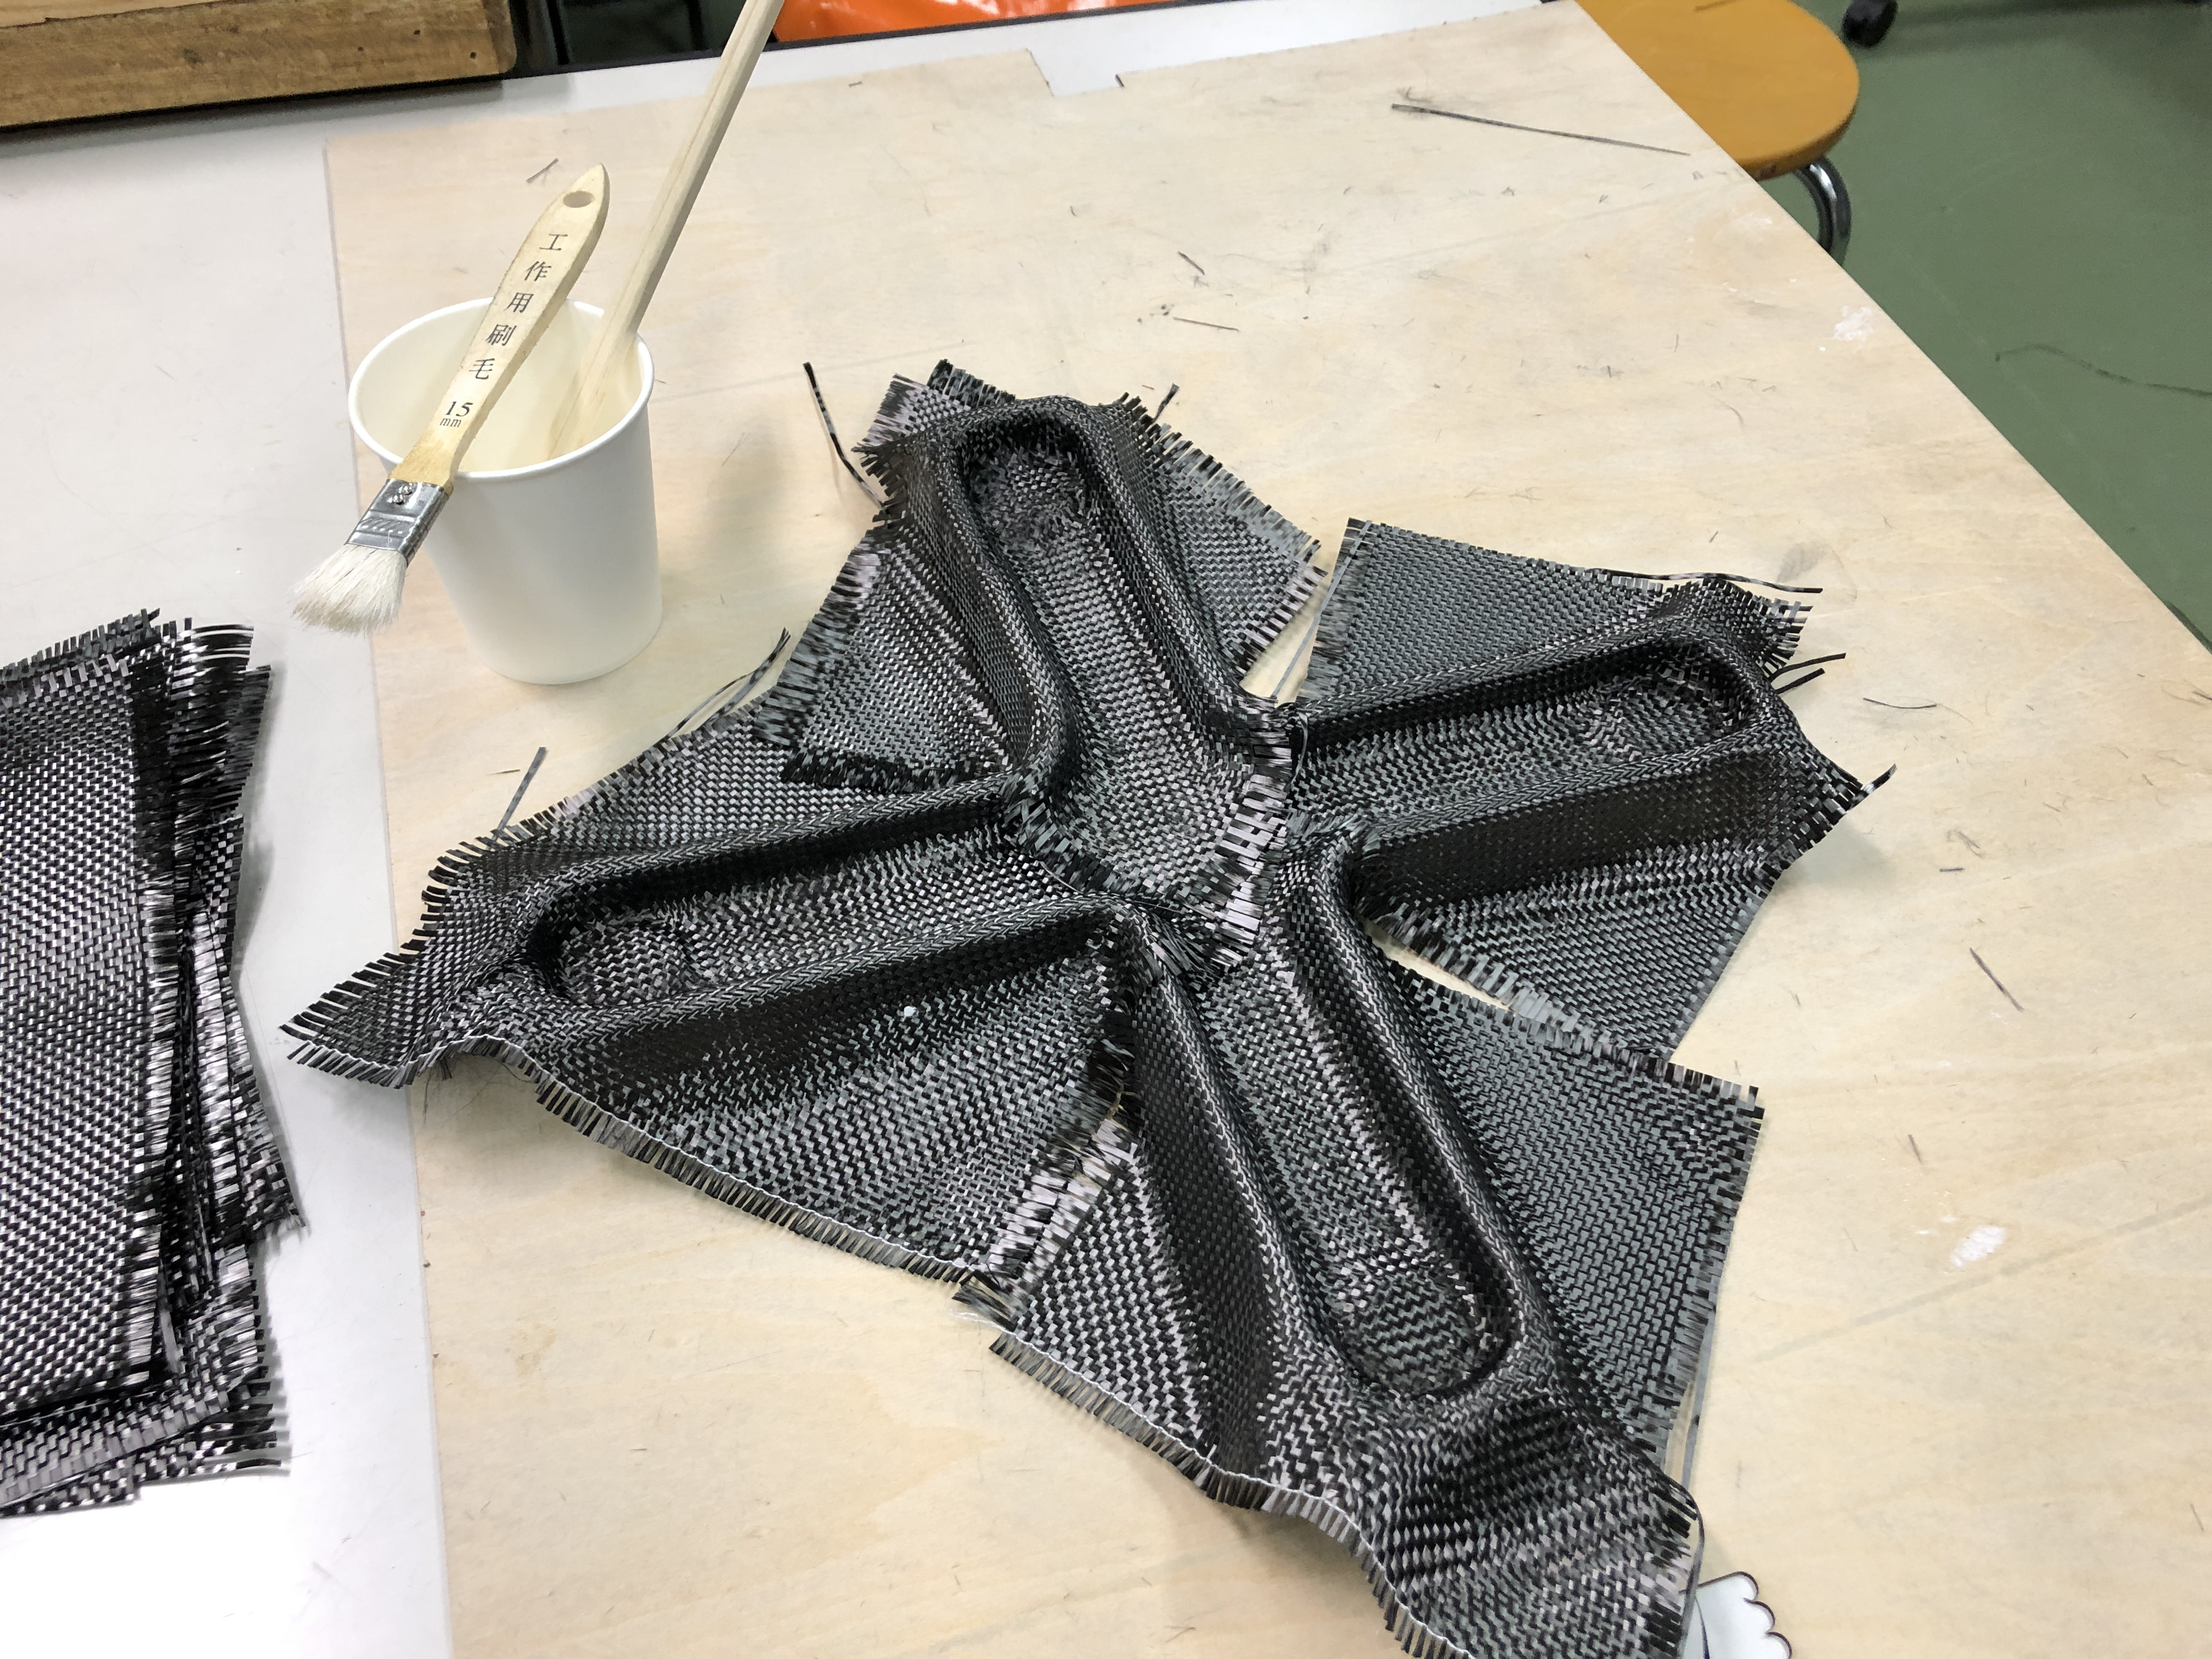
\includegraphics[width=120mm]{img/11.JPG}
    \end{center}
  \caption{四分割された}
 \label{fig:robot}
\end{figure}

\begin{figure}[htbp]
  \begin{center}
    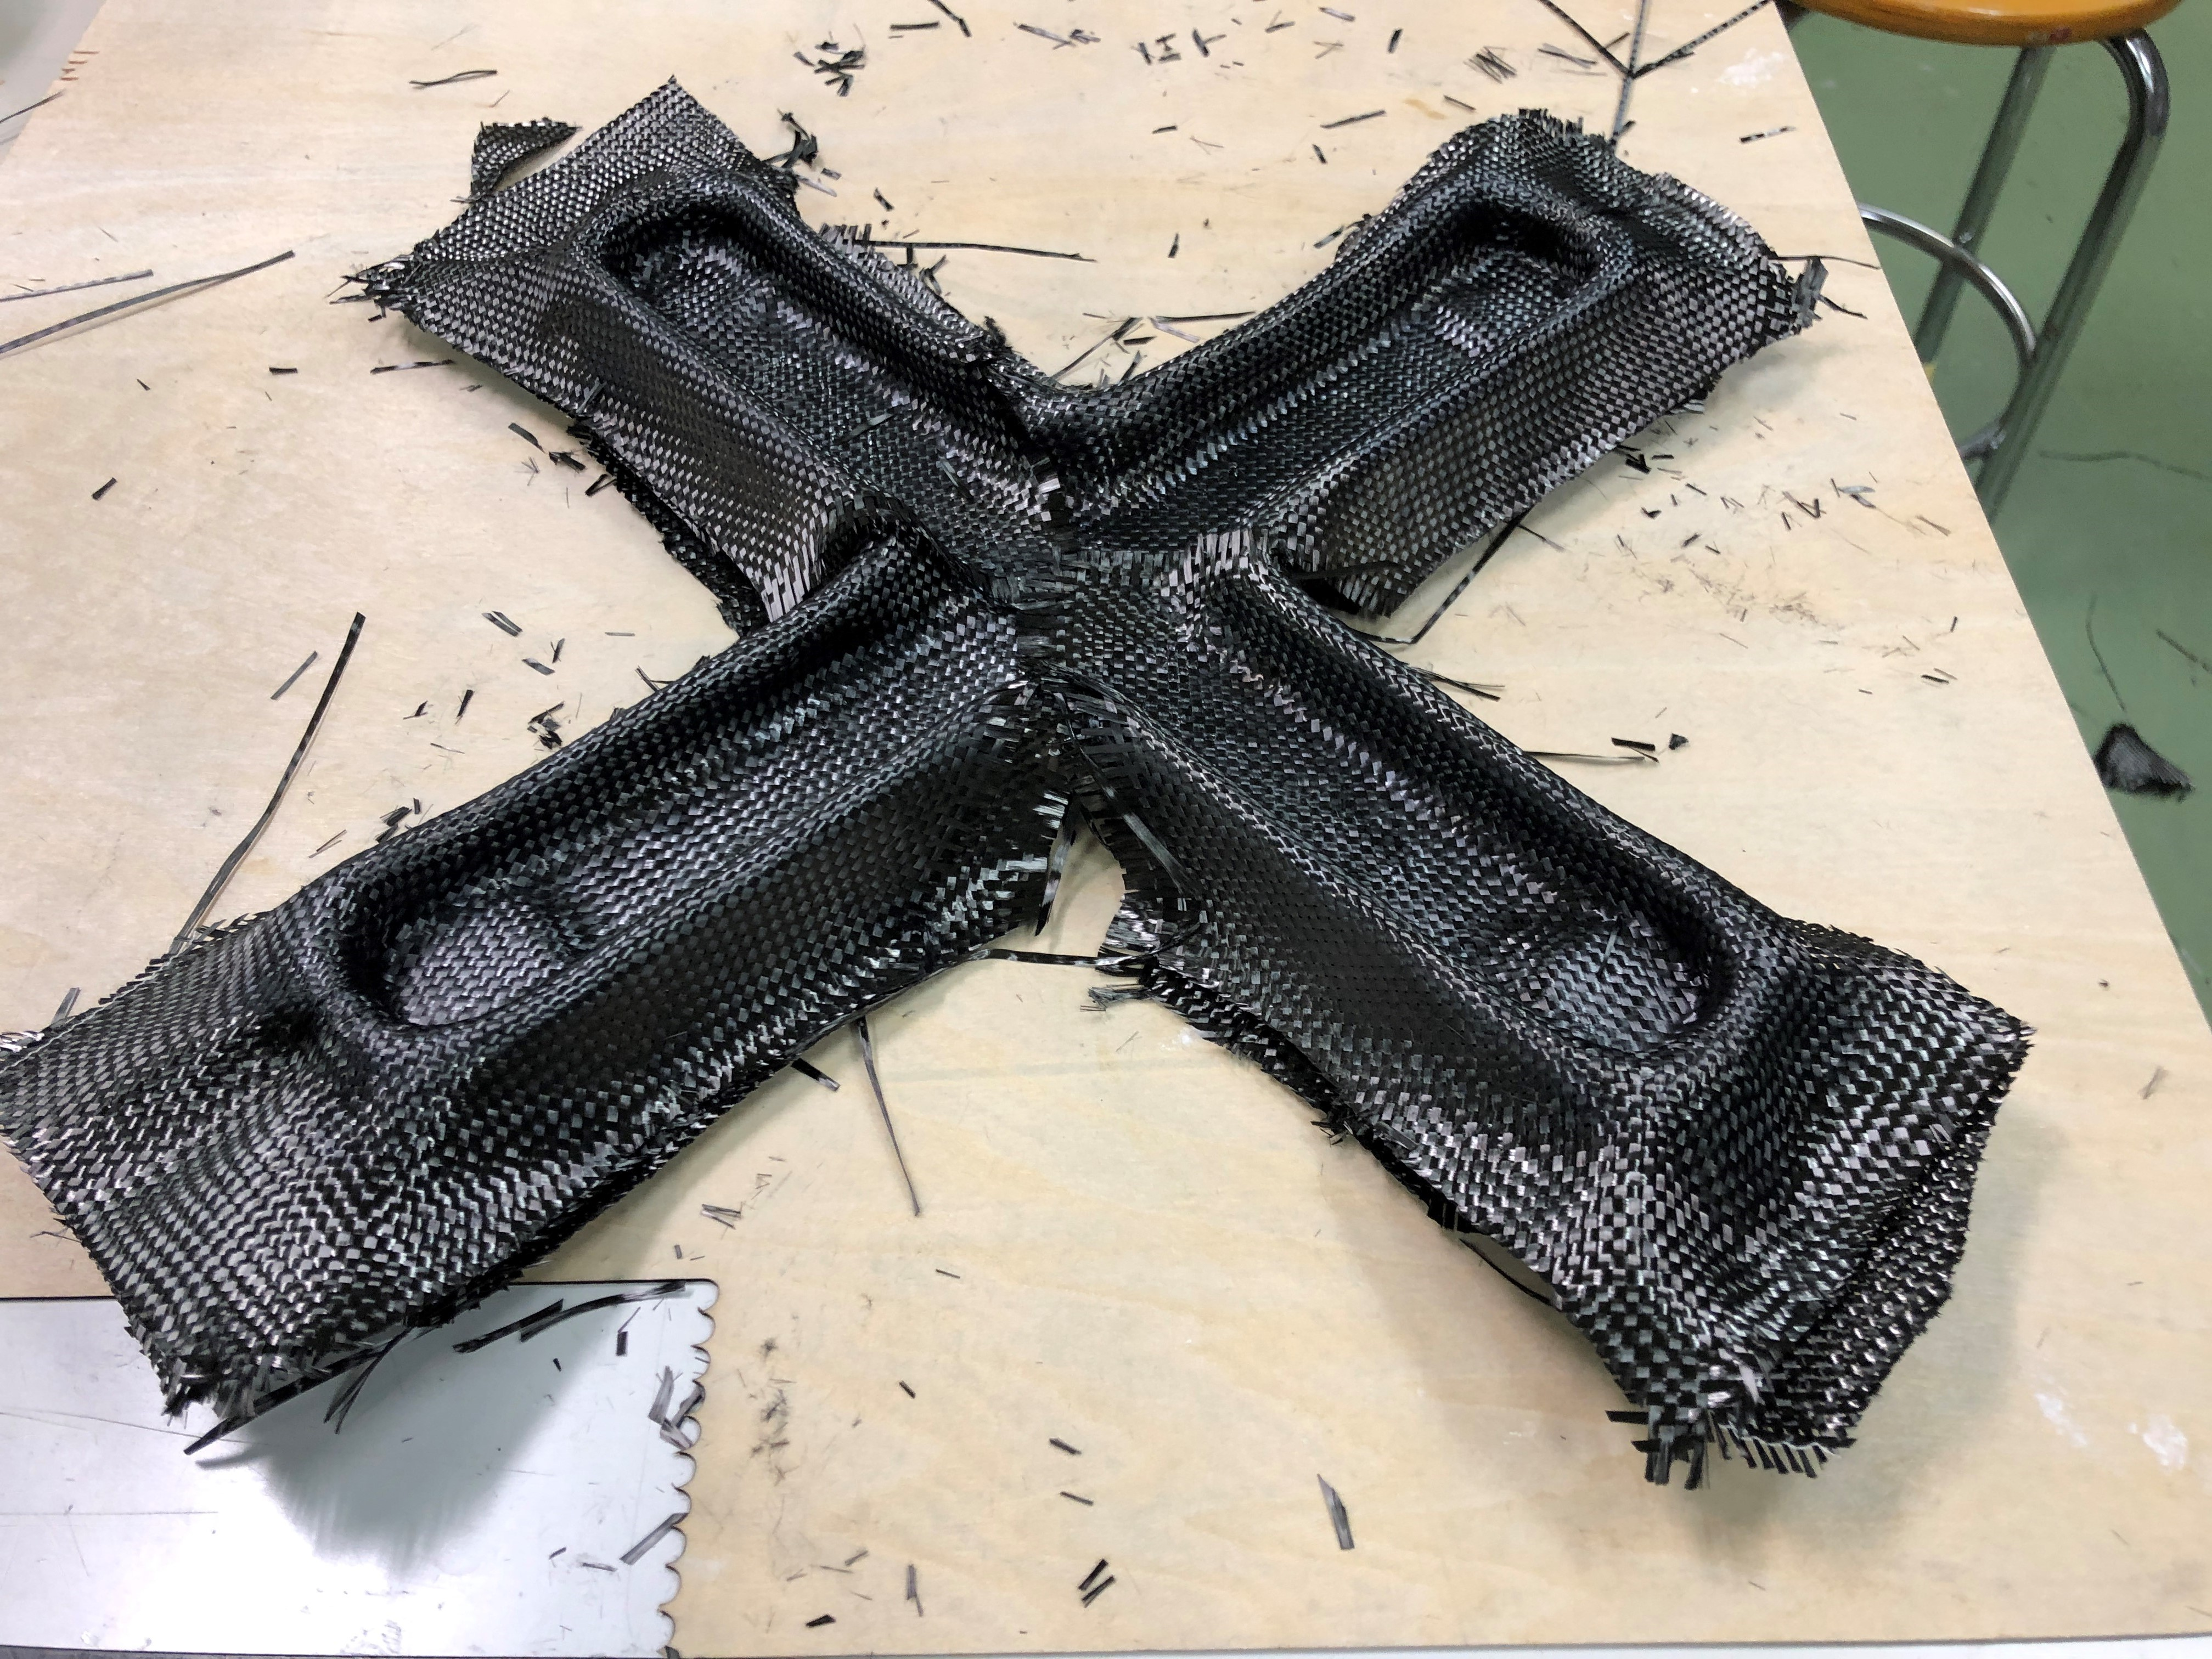
\includegraphics[width=120mm]{img/12.JPG}
    \end{center}
  \caption{硬化剤を塗られ積層されたカーボンシート}
 \label{fig:robot}
\end{figure}

\section{真空引き作業}
圧縮作業には,吸引機として掃除機とビニールポリ袋を用いて作業行った.積層作業を終えたものをビニールポリ袋に入れる.その後吸引のためのノズルを通す部分以外をアイロンで温め溶着させる.その後掃除機で圧縮作業を行っていく.圧縮の際に一気に空気を抜いていくのではなく,徐々に空気量を調整していきながらポリ袋を型の形に添わせながら空気を抜いてゆく.また型の角がポリ袋を傷つけないかを気を付けながら完全に空気を抜いていく.最終的にノズルを抜いていき,すべてを抜ききる手前でアイロンで溶着をさせ圧縮作業が完了する.

\begin{figure}[htbp]
  \begin{center}
    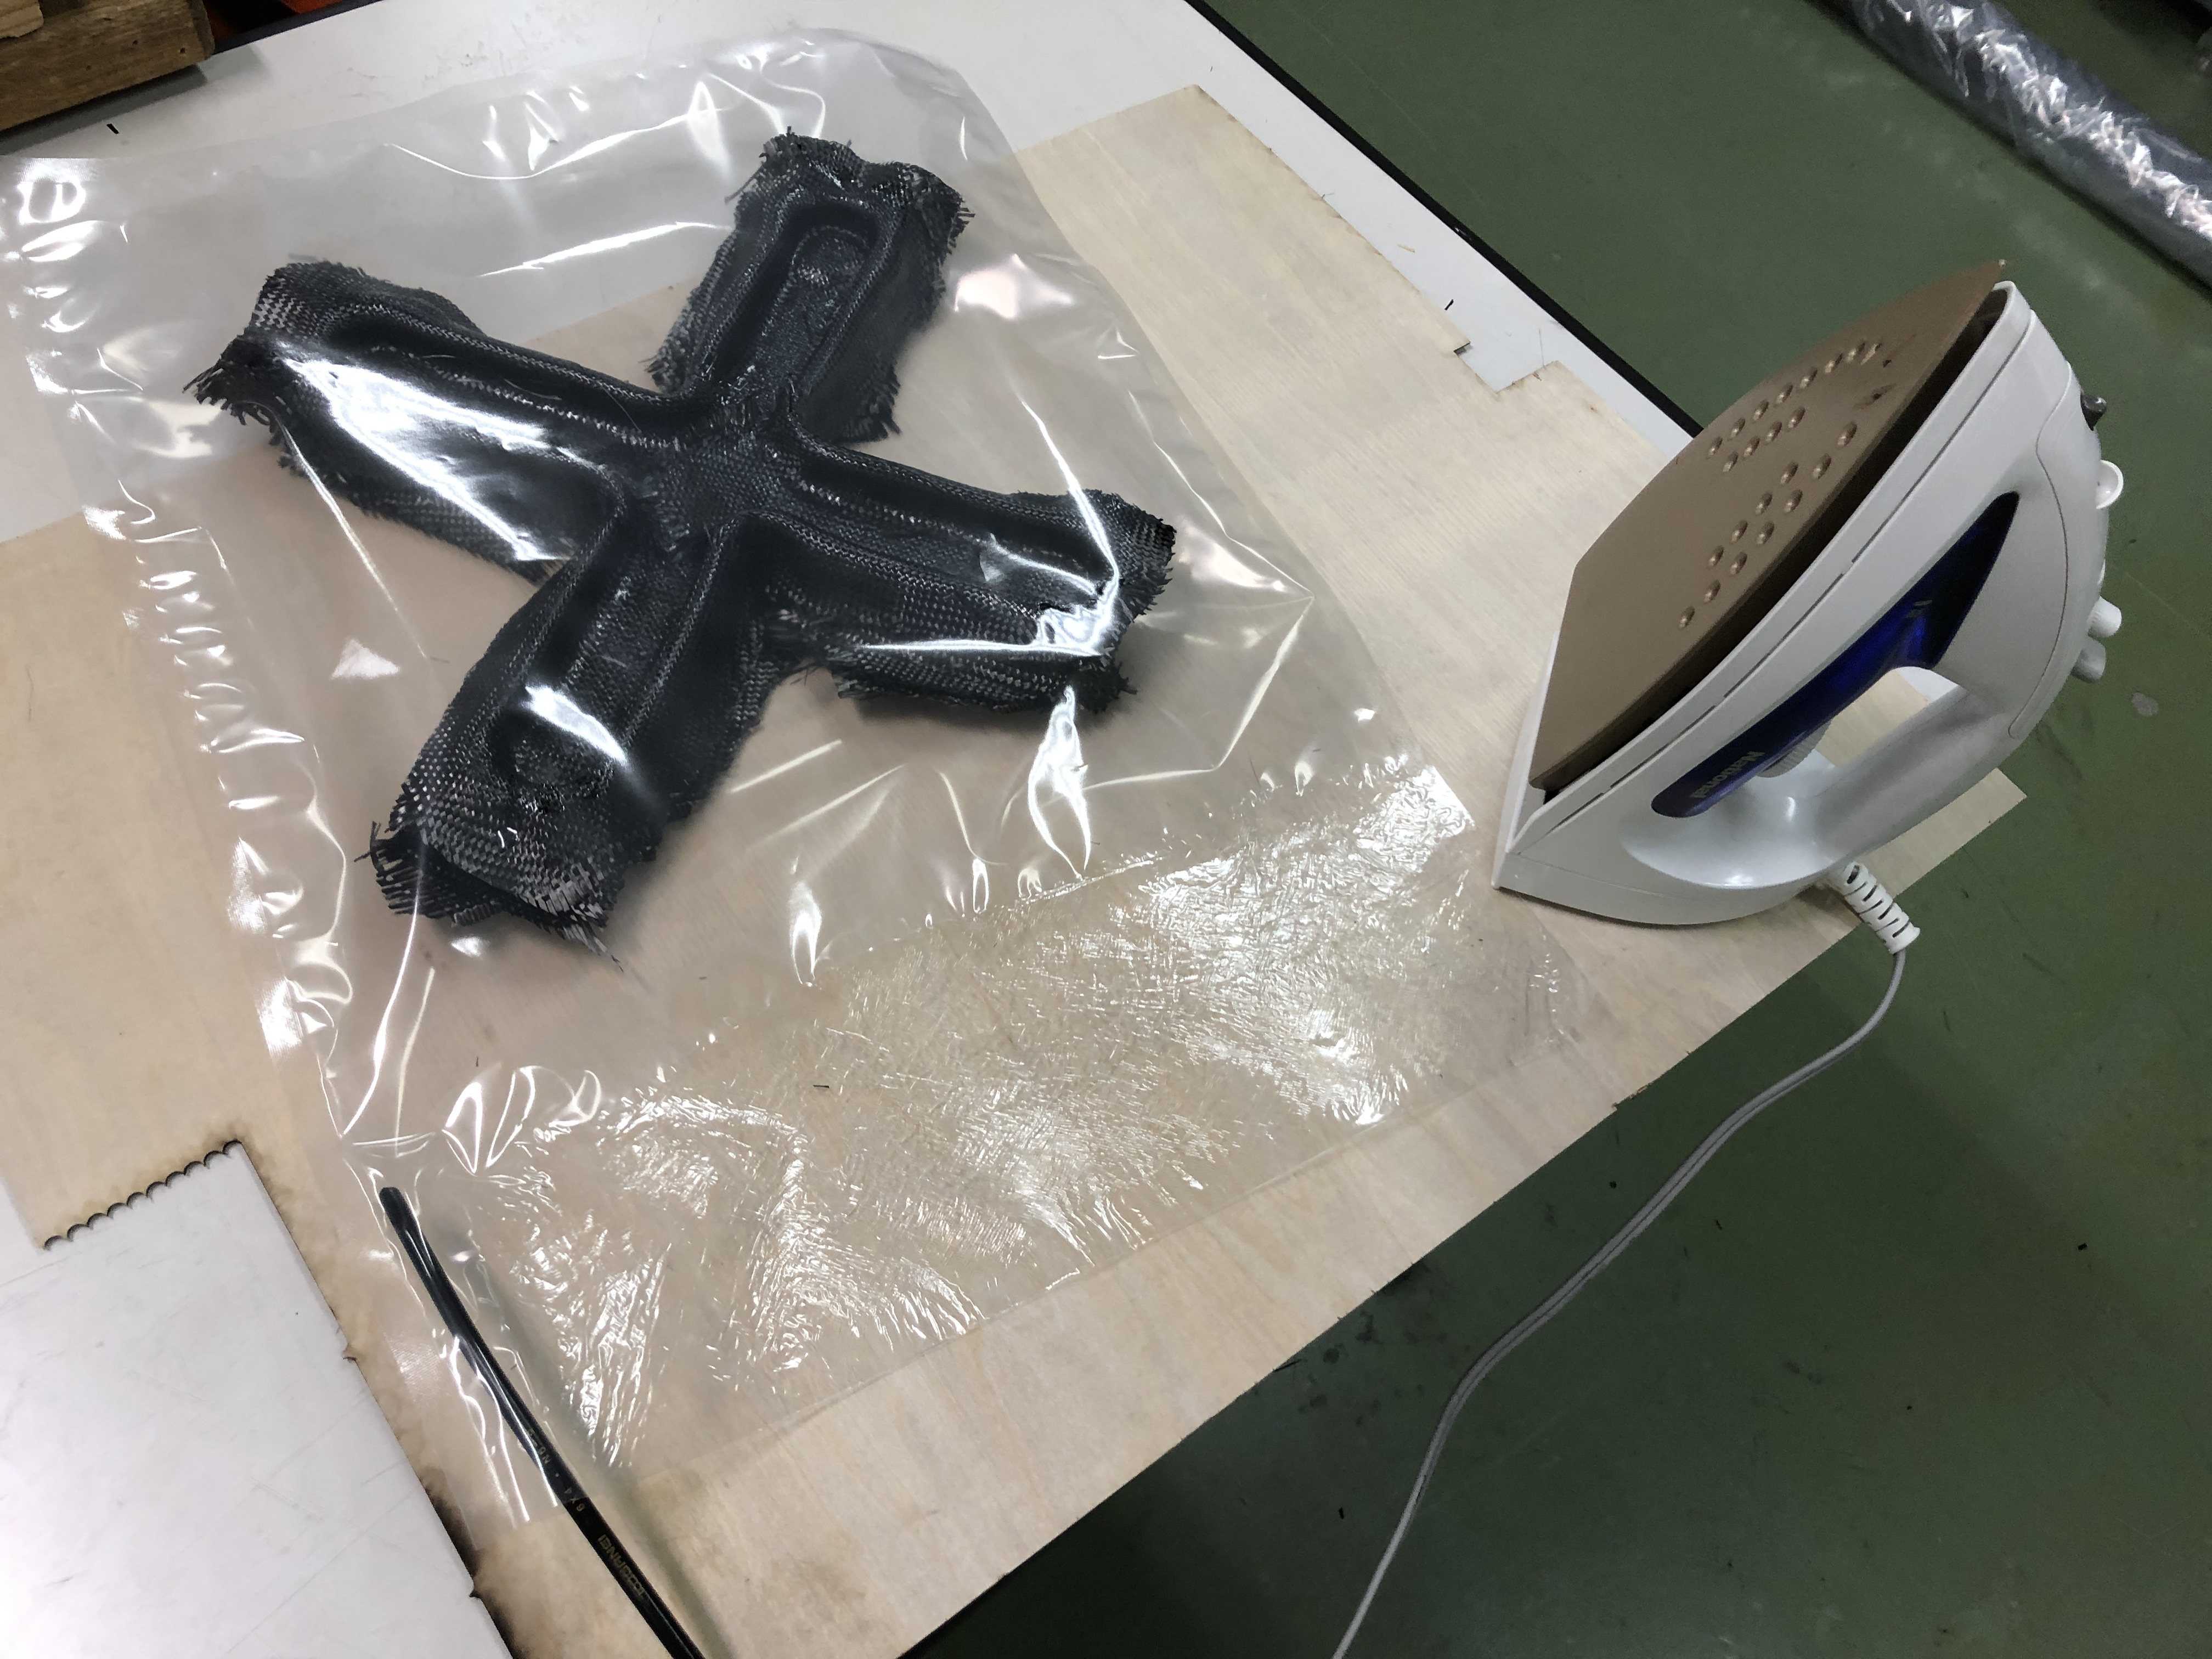
\includegraphics[width=120mm]{img/13.JPG}
    \end{center}
  \caption{真空引き前のフレーム}
 \label{fig:robot}
\end{figure}

\begin{figure}[htbp]
  \begin{center}
    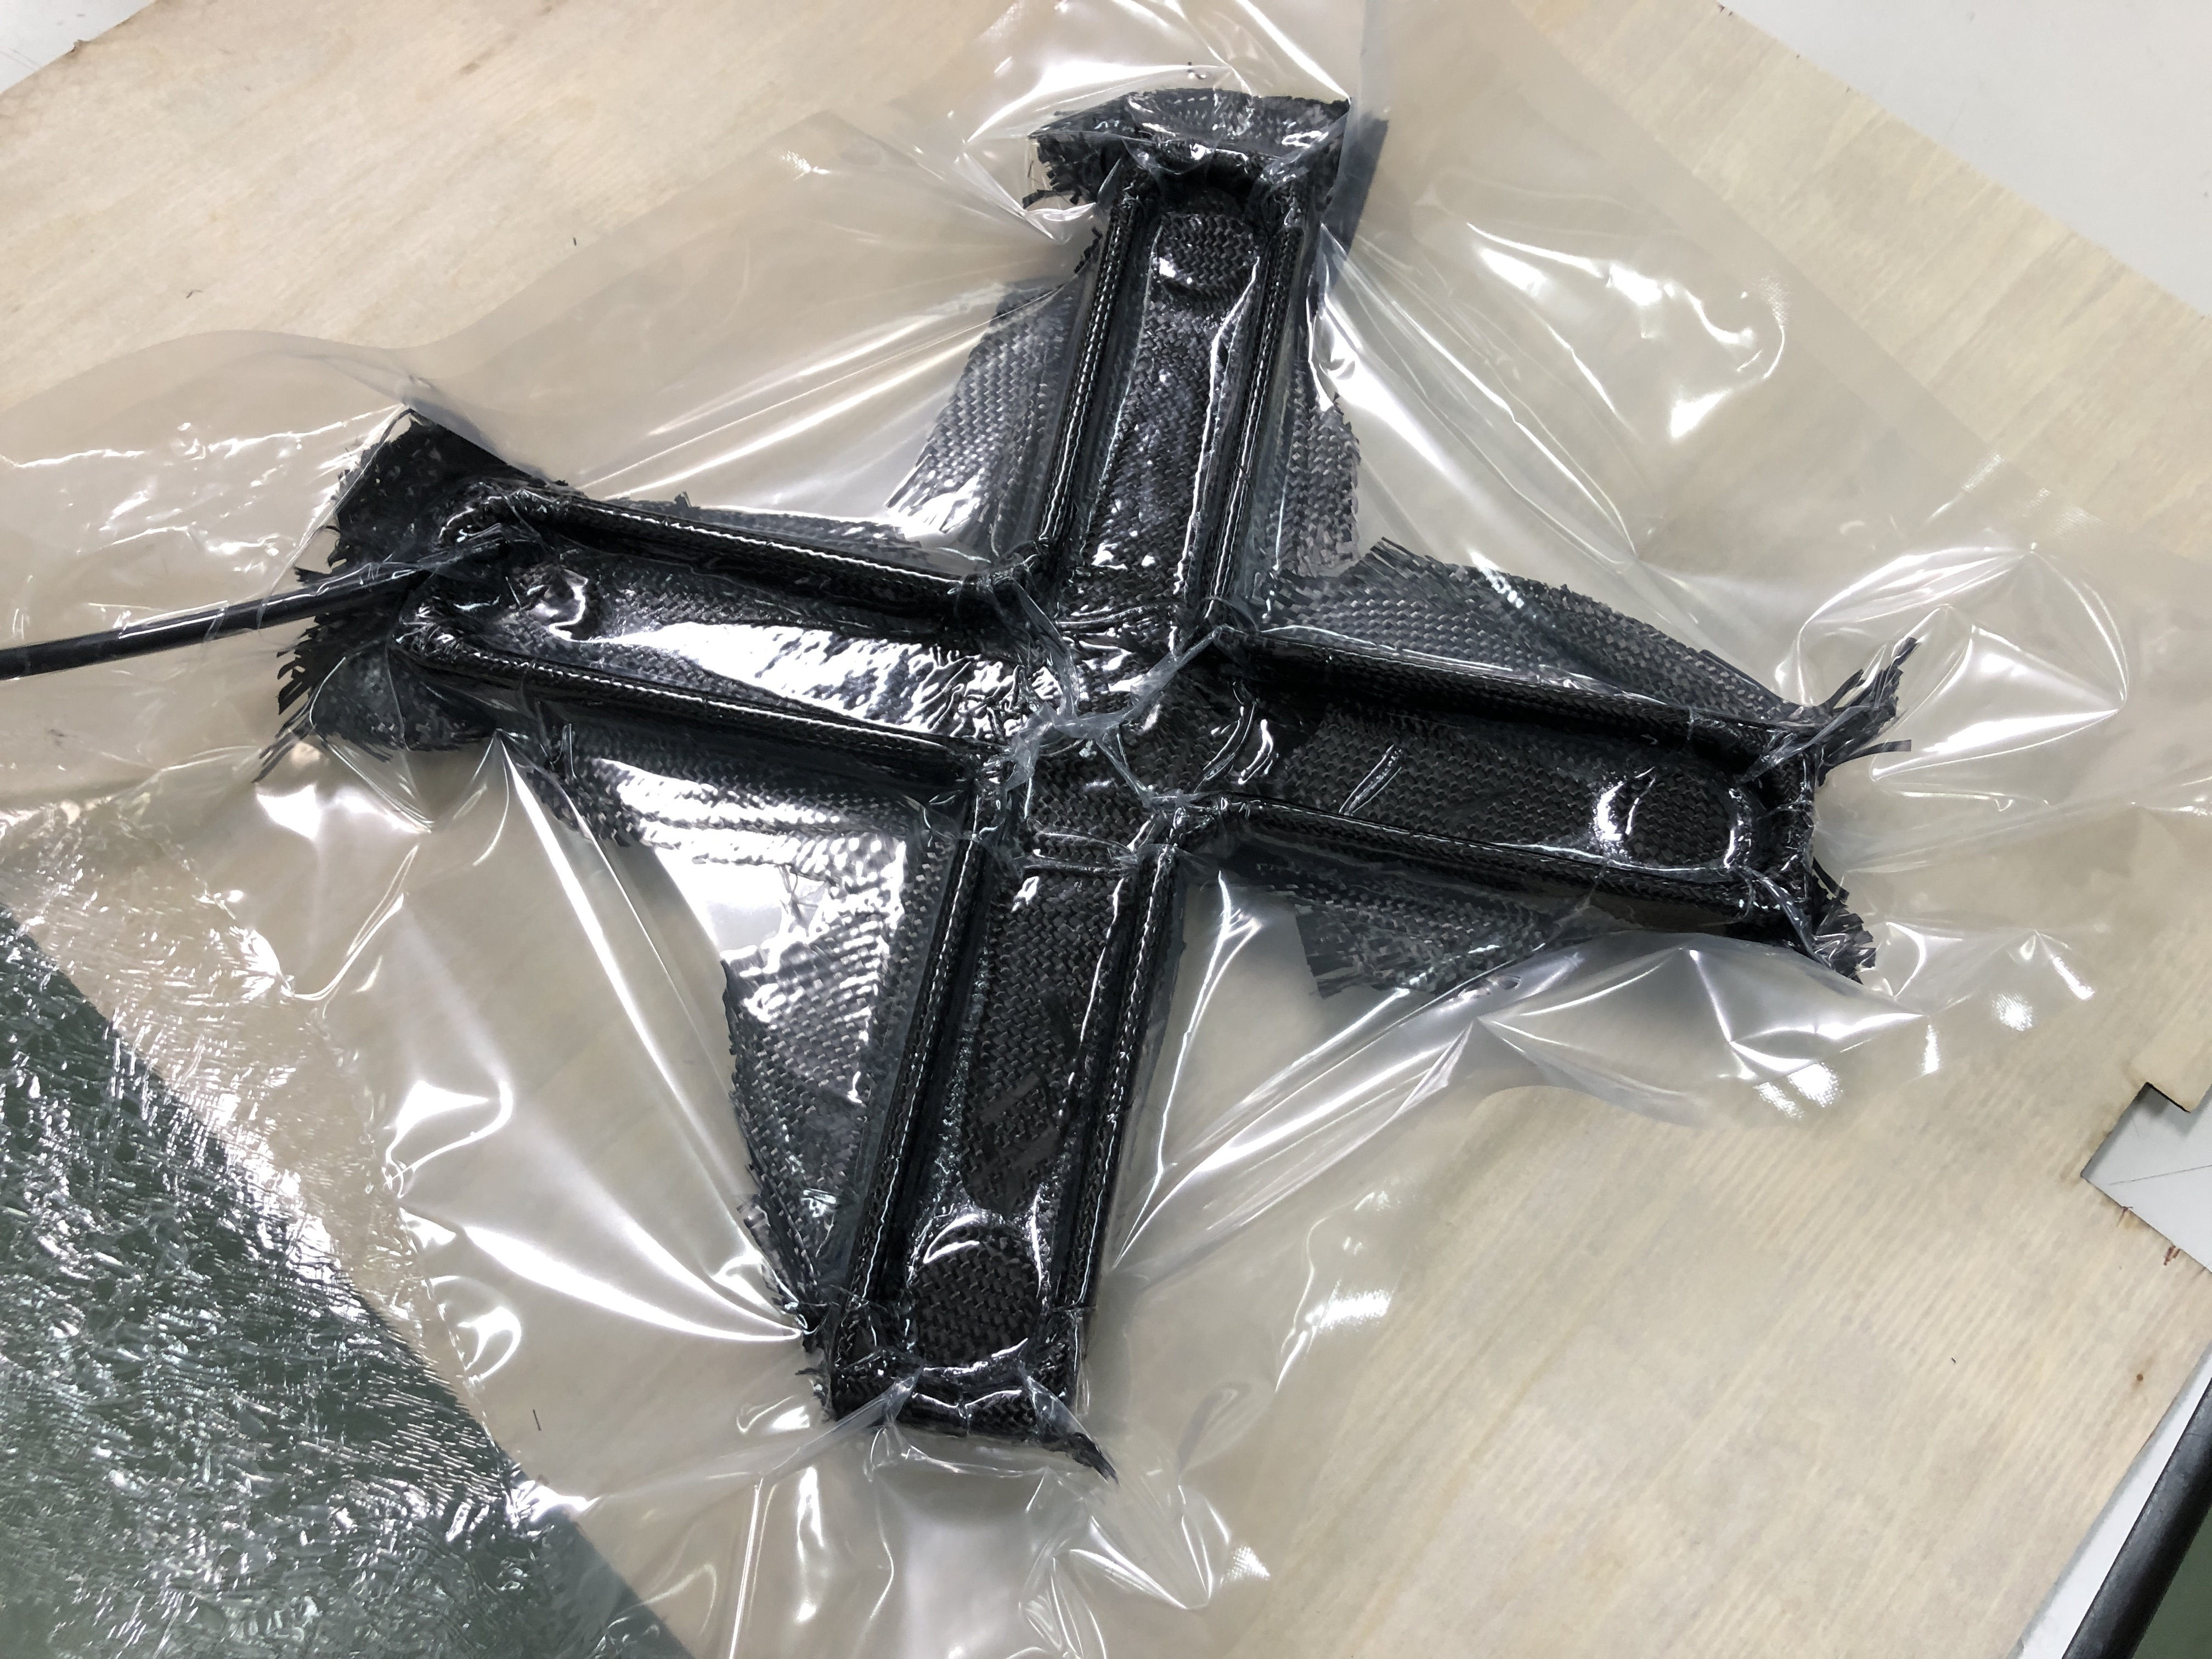
\includegraphics[width=120mm]{img/14.JPG}
    \end{center}
  \caption{真空引き後アイロンで密閉されたフレーム}
 \label{fig:robot}
\end{figure}

\section{バリ取り,ヤスリ掛け}
24時間以上が経過し完全移行化したフレームは,型から取り外しバリを糸ノコで切り落とし,やすり掛けを行い完成となる.

\begin{figure}[htbp]
  \begin{center}
    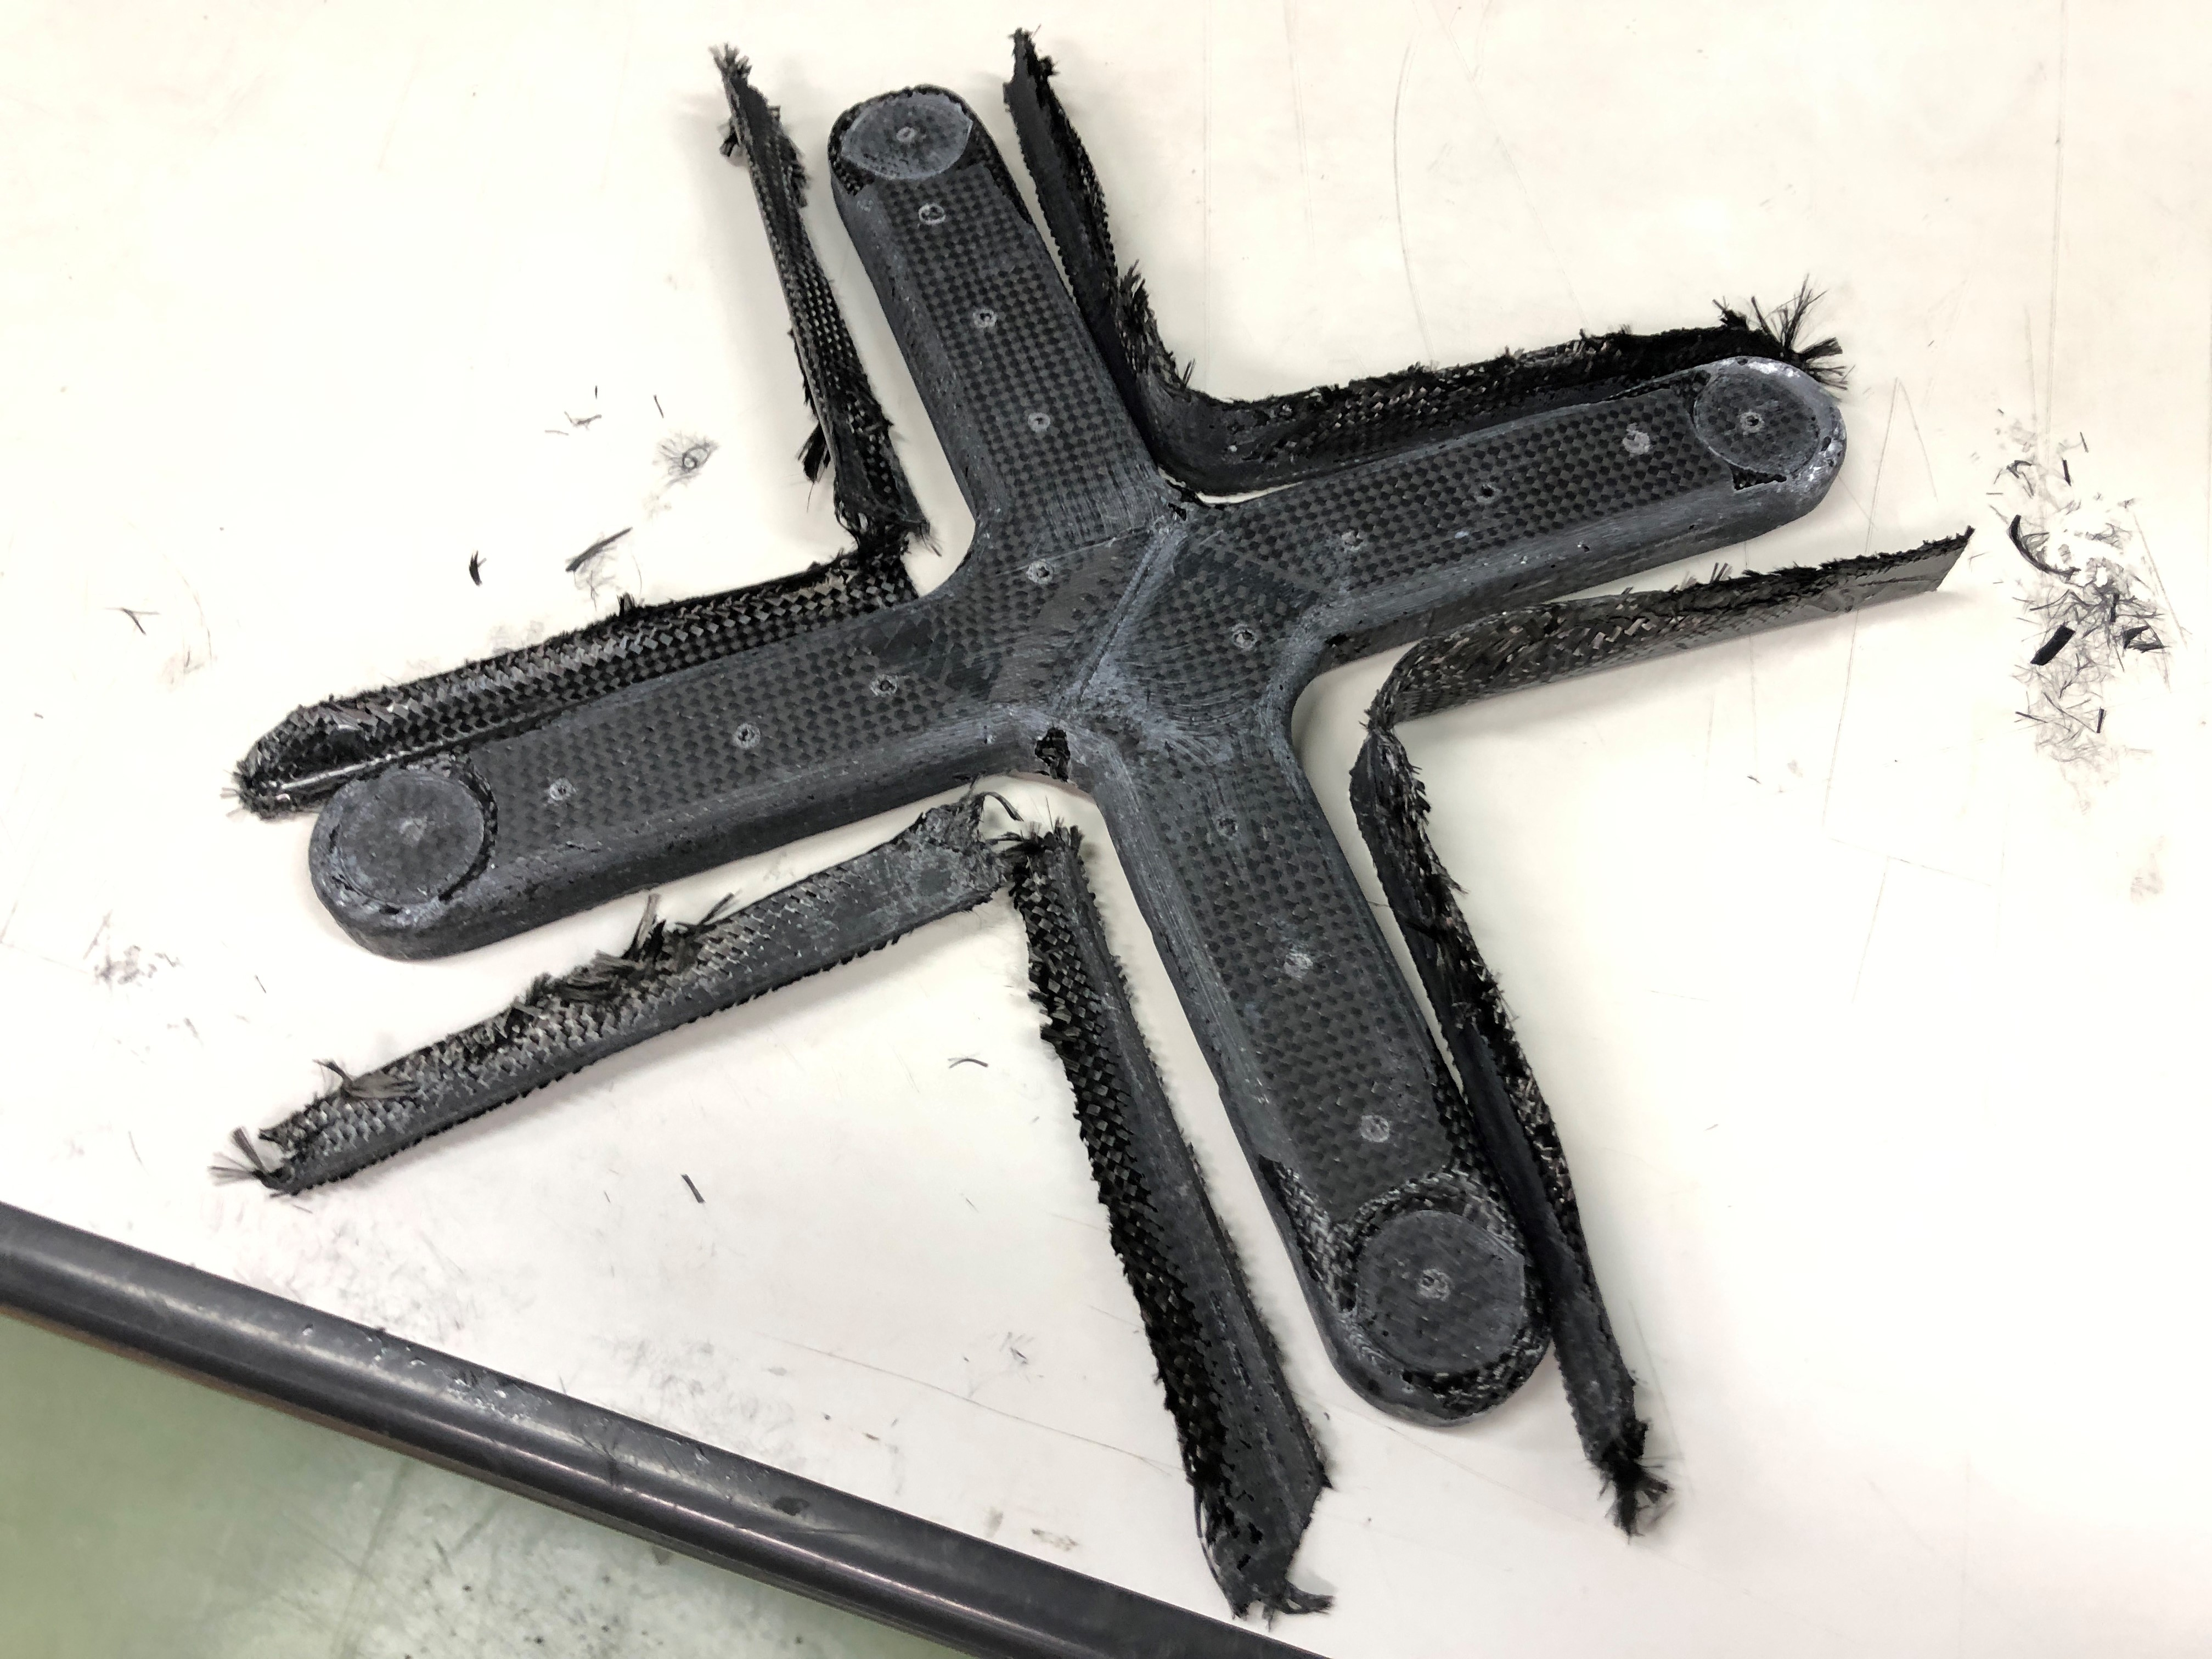
\includegraphics[width=120mm]{img/15.JPG}
    \end{center}
  \caption{バリ取り後のフレーム}
 \label{fig:robot}
\end{figure}

\begin{figure}[htbp]
  \begin{center}
    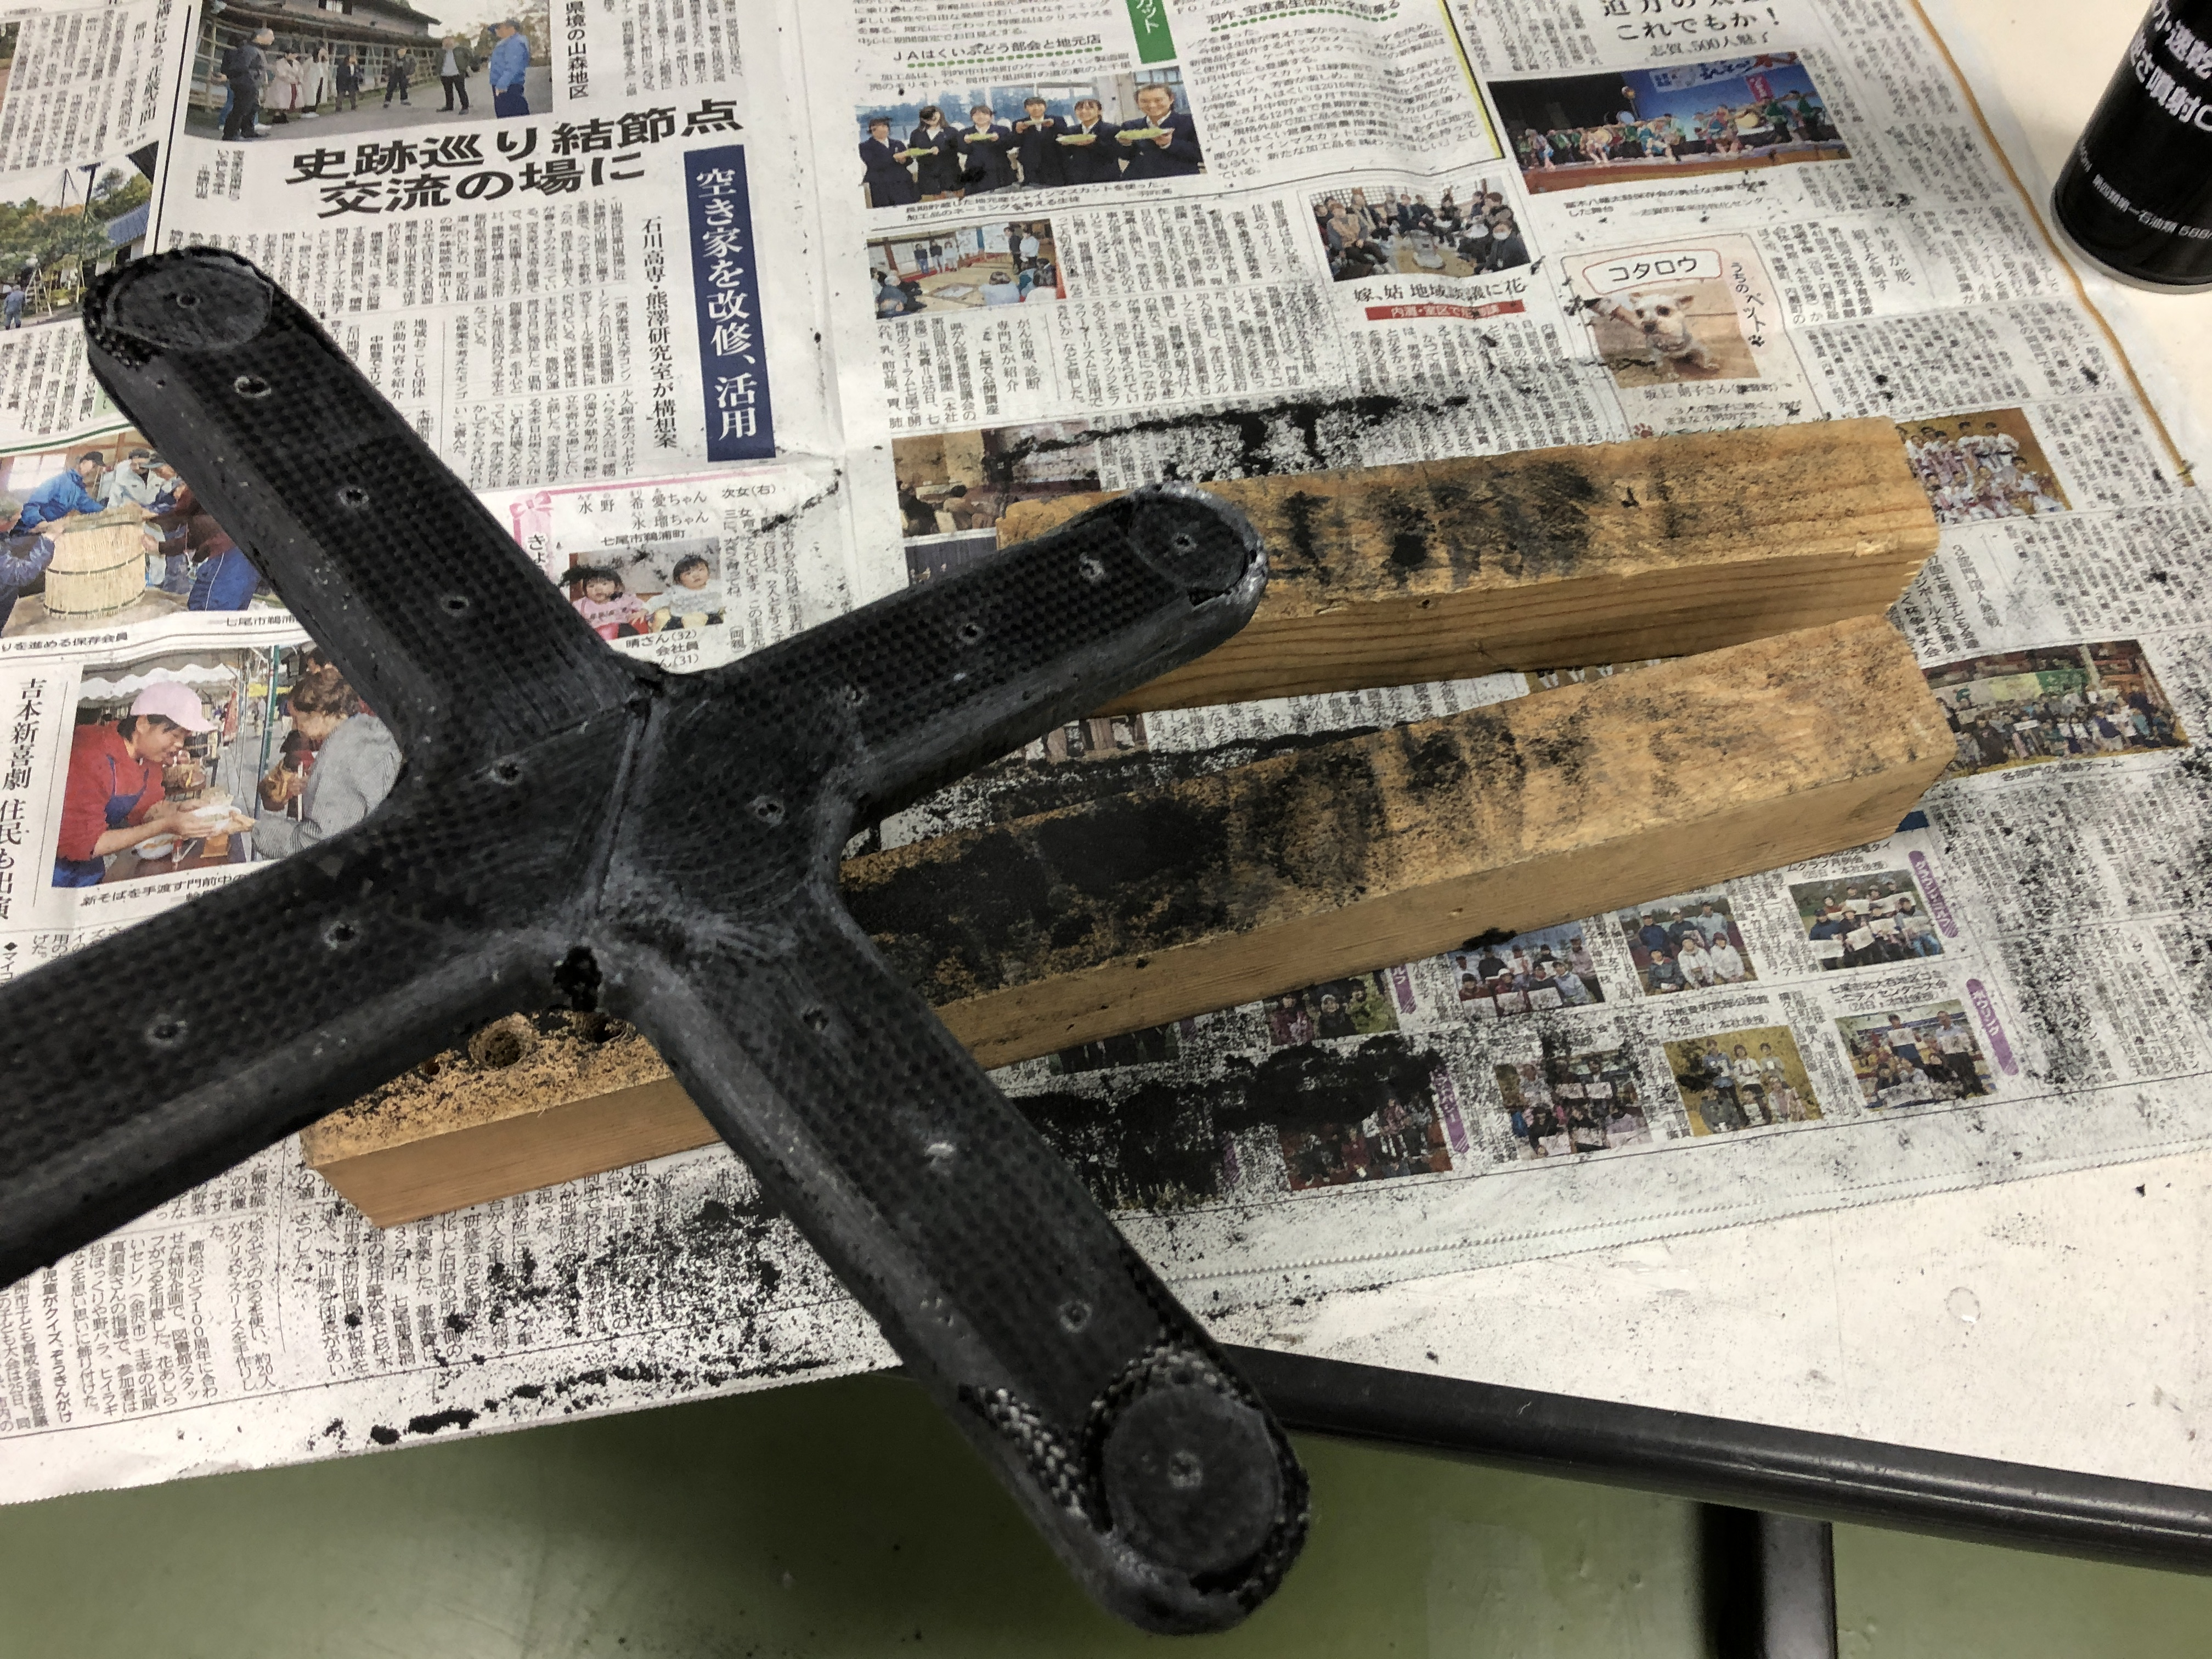
\includegraphics[width=120mm]{img/16.JPG}
    \end{center}
  \caption{ヤスリをかけ仕上げられたフレーム}
 \label{fig:robot}
\end{figure}

\section{立体フレーム製作過程においてのまとめ}
\subsection{離型剤について}
立体フレーム製作において積層硬化後,離型に車用ワックスとエポキシ樹脂用スプレー型離型剤を用いた,ワックスは代用品ではあるが樹脂と型との間に膜の役割として塗ることができるため比較的容易に離型することができる.ポリプロピレン製のフィルムは,立体の複雑な形に対しての柔軟性がなかったため使用をしなかった,また,ワックスを用いての離型後も表面状態が異なった.
平面積層時同様にスプレー型の専用のものを使った場合,表面はつやがないマットな仕上がりとなった,しかし,散布する量にむらがあったり,量が多くなりすぎると表面に固着してしまい仕上がり面が綺麗にならなかった.
それに対しワックスを用いた場合は,仕上がりは艶のない面となった.
ワックスは固形であるため,手作業で量を調節しながら塗り込めるので,スプレー式より最適であった,

\subsection{樹脂吸着シートについて}
立体積層においては平面積層に比べ多量の硬化剤を用いる.よって積層後に雌型の底の部分に樹脂の溜まりができてしまう.そのため余分な樹脂を除去するために専用に吸着シートを用いた.しかし積層時にしわになってしまうとカーボンクロスに巻き込まれてしまい綺麗な積層が行えなかったため使用はしなかった.樹脂がたまる対策として,雌型に穴をあけて溜まらないように加工を施した.

\begin{figure}[htbp]
  \begin{center}
    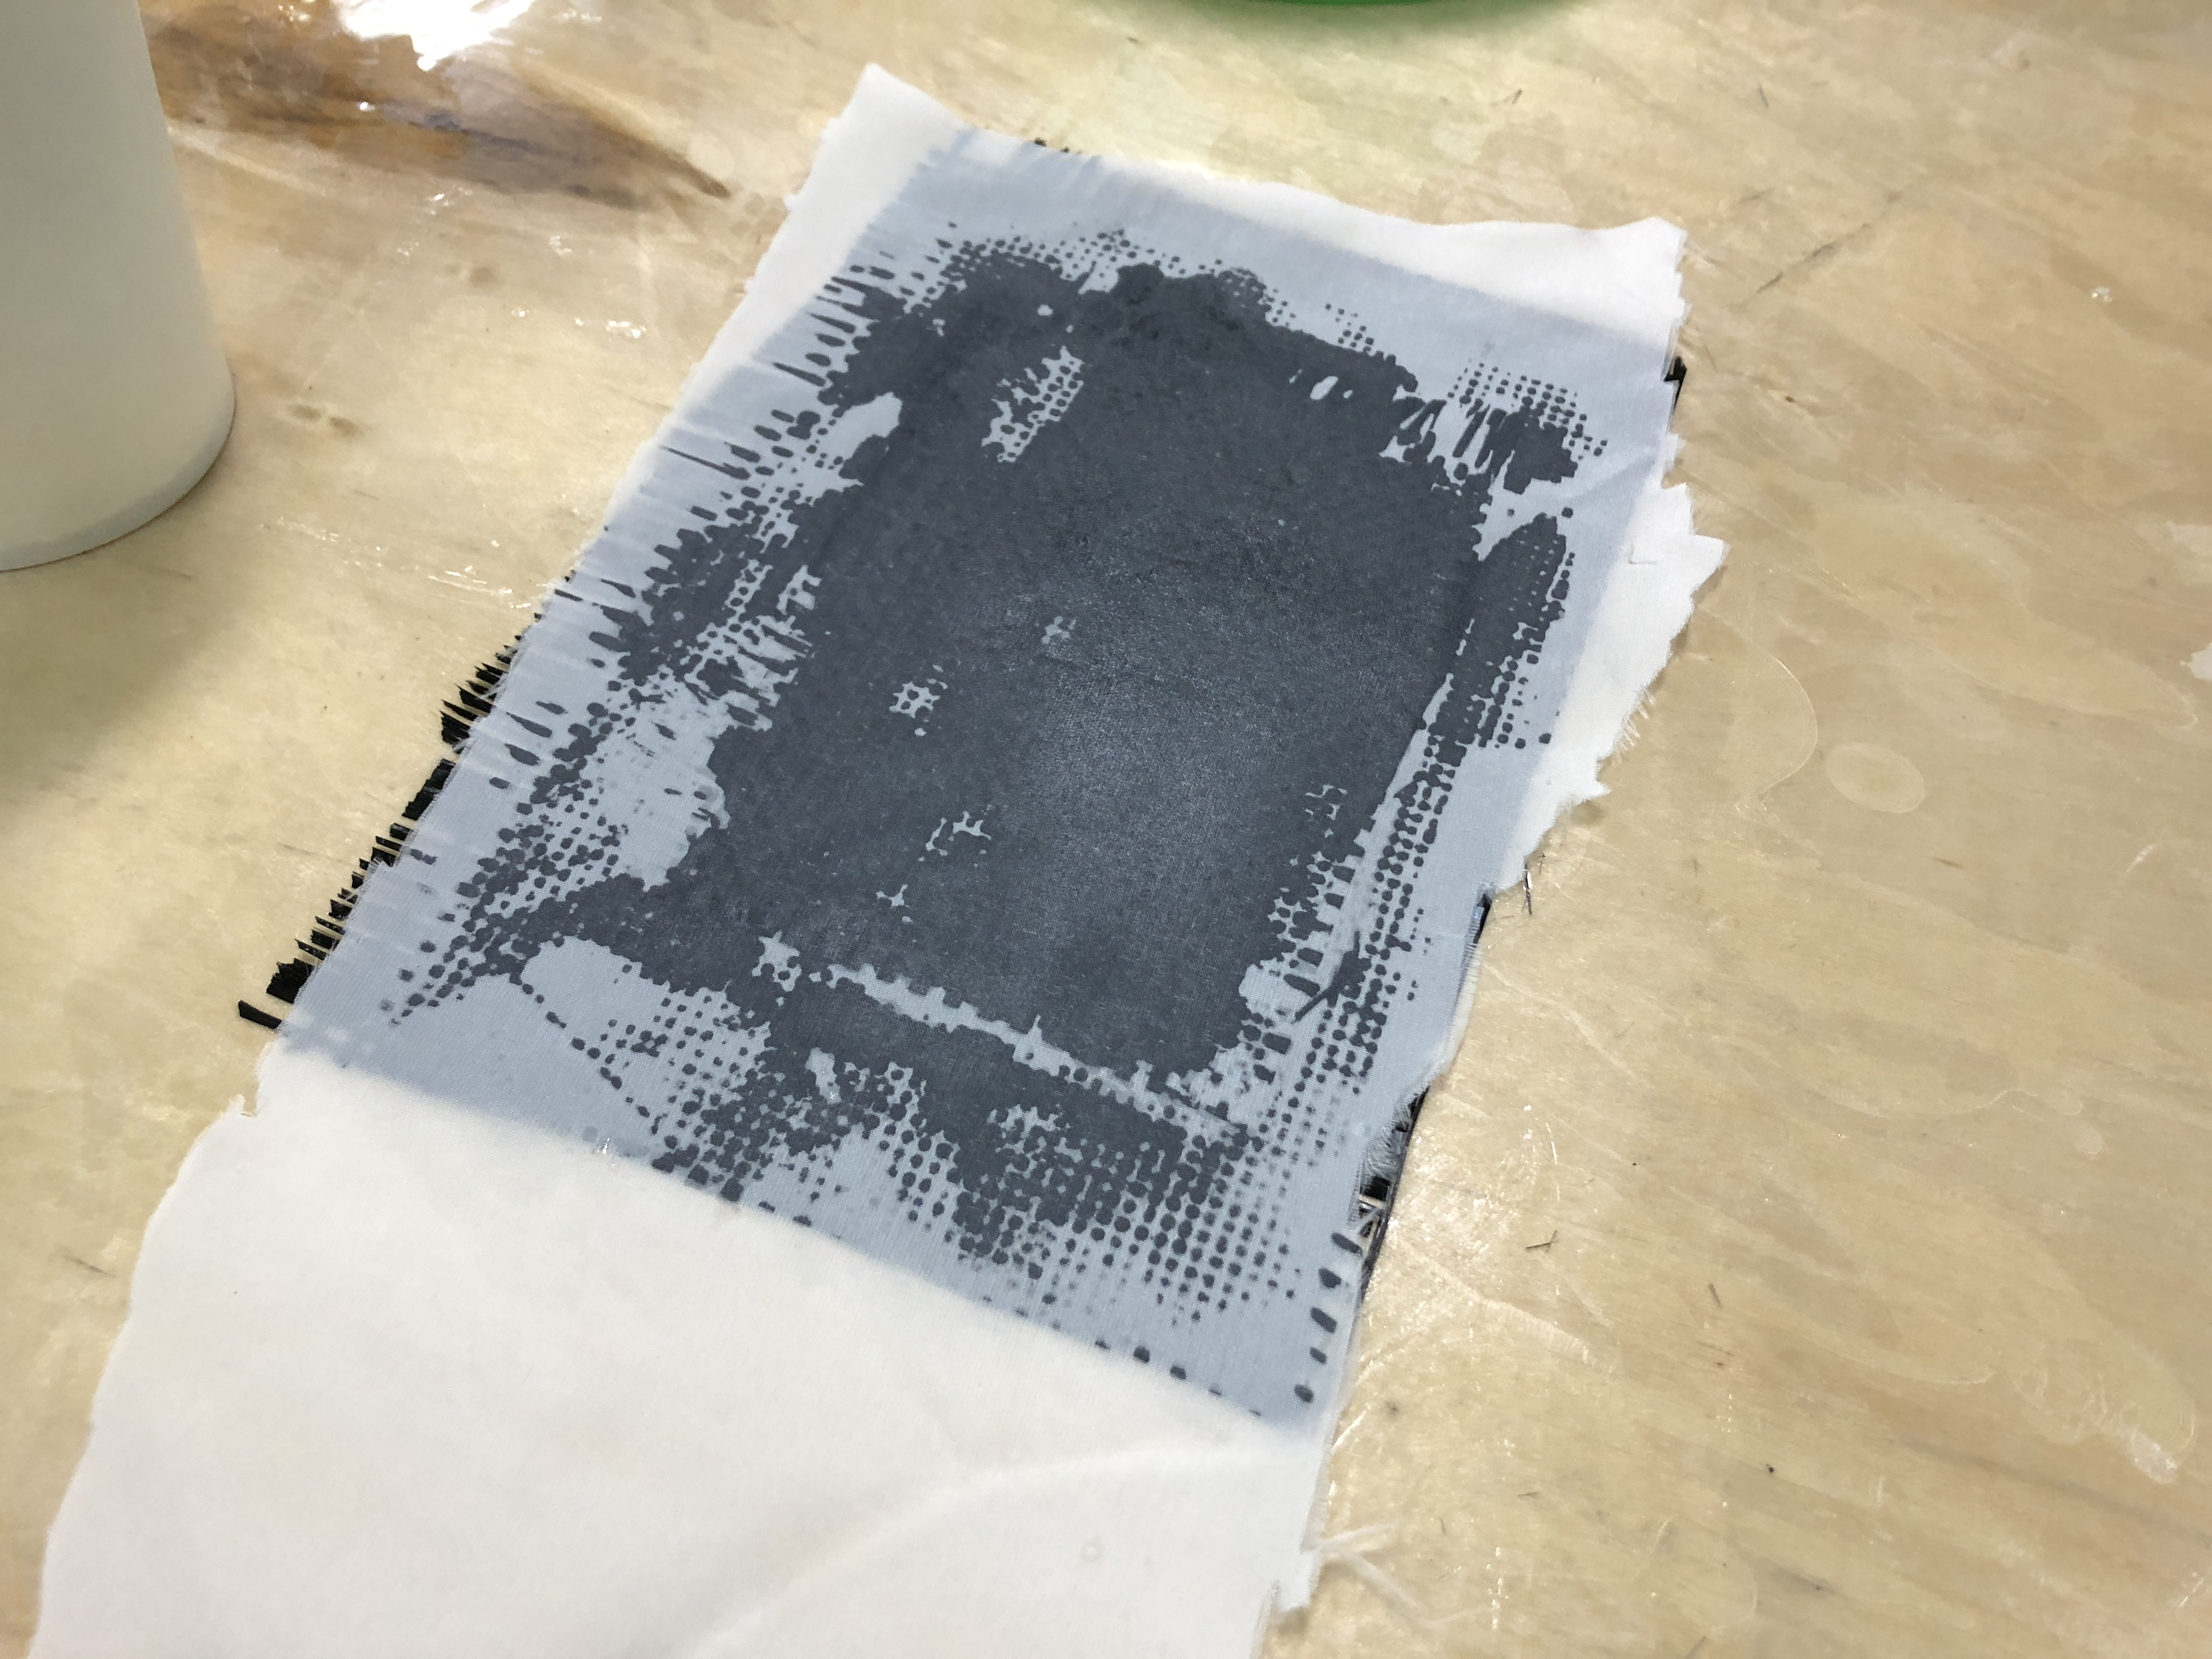
\includegraphics[width=120mm]{img/25.JPG}
    \end{center}
  \caption{樹脂吸着シート}
 \label{fig:robot}
\end{figure}

\begin{figure}[htbp]
  \begin{center}
    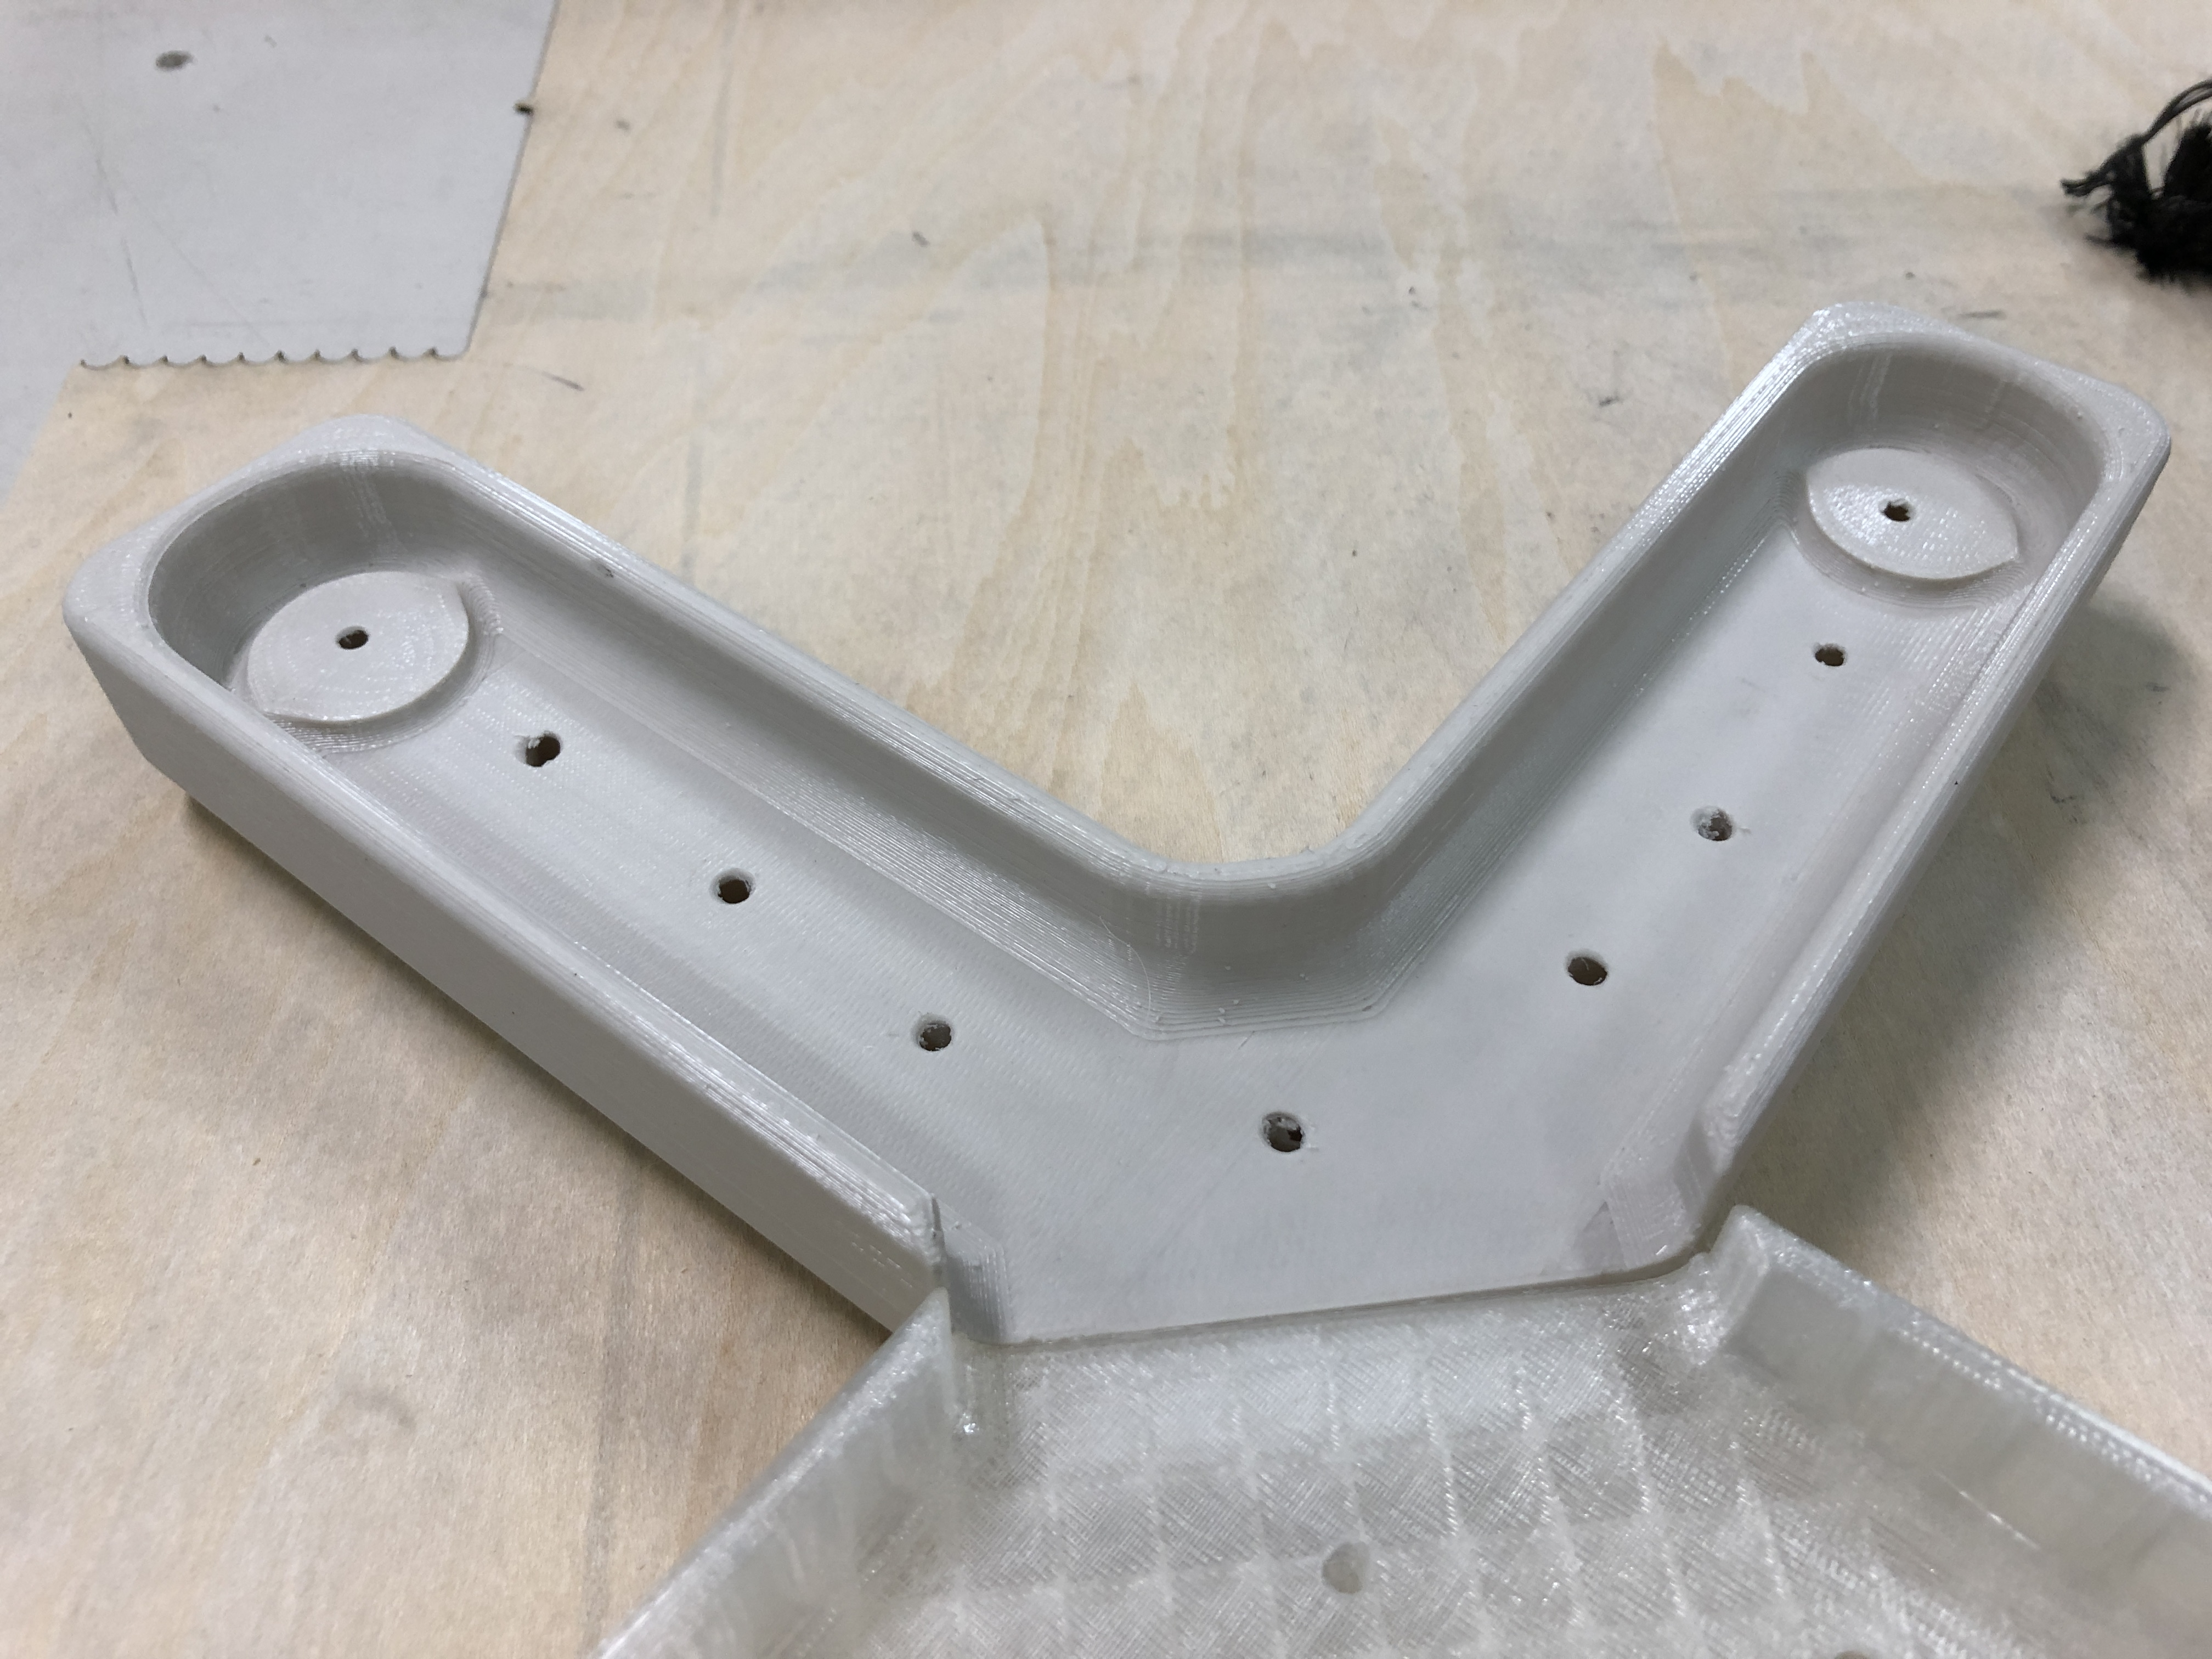
\includegraphics[width=120mm]{img/26.JPG}
    \end{center}
  \caption{穴あけ加工された雌型}
 \label{fig:robot}
\end{figure}

\subsection{雄型,雌型を用いての成型について}
真空引きで成型を行う以前に,雄型と雌型を用いての成型方法を試みた.雌型にカーボンシート,樹脂吸着シートを積層し,雄型をはめ合わせおもりをのせて成型する.しかし,雄型と雌型のはめ合いが相枚数次第で変わってしまう.そのためはめ合わせがきつくなりすぎると,硬化後の離型がとても困難だったため真空引きが立体積層において適している.

\begin{figure}[htbp]
  \begin{center}
    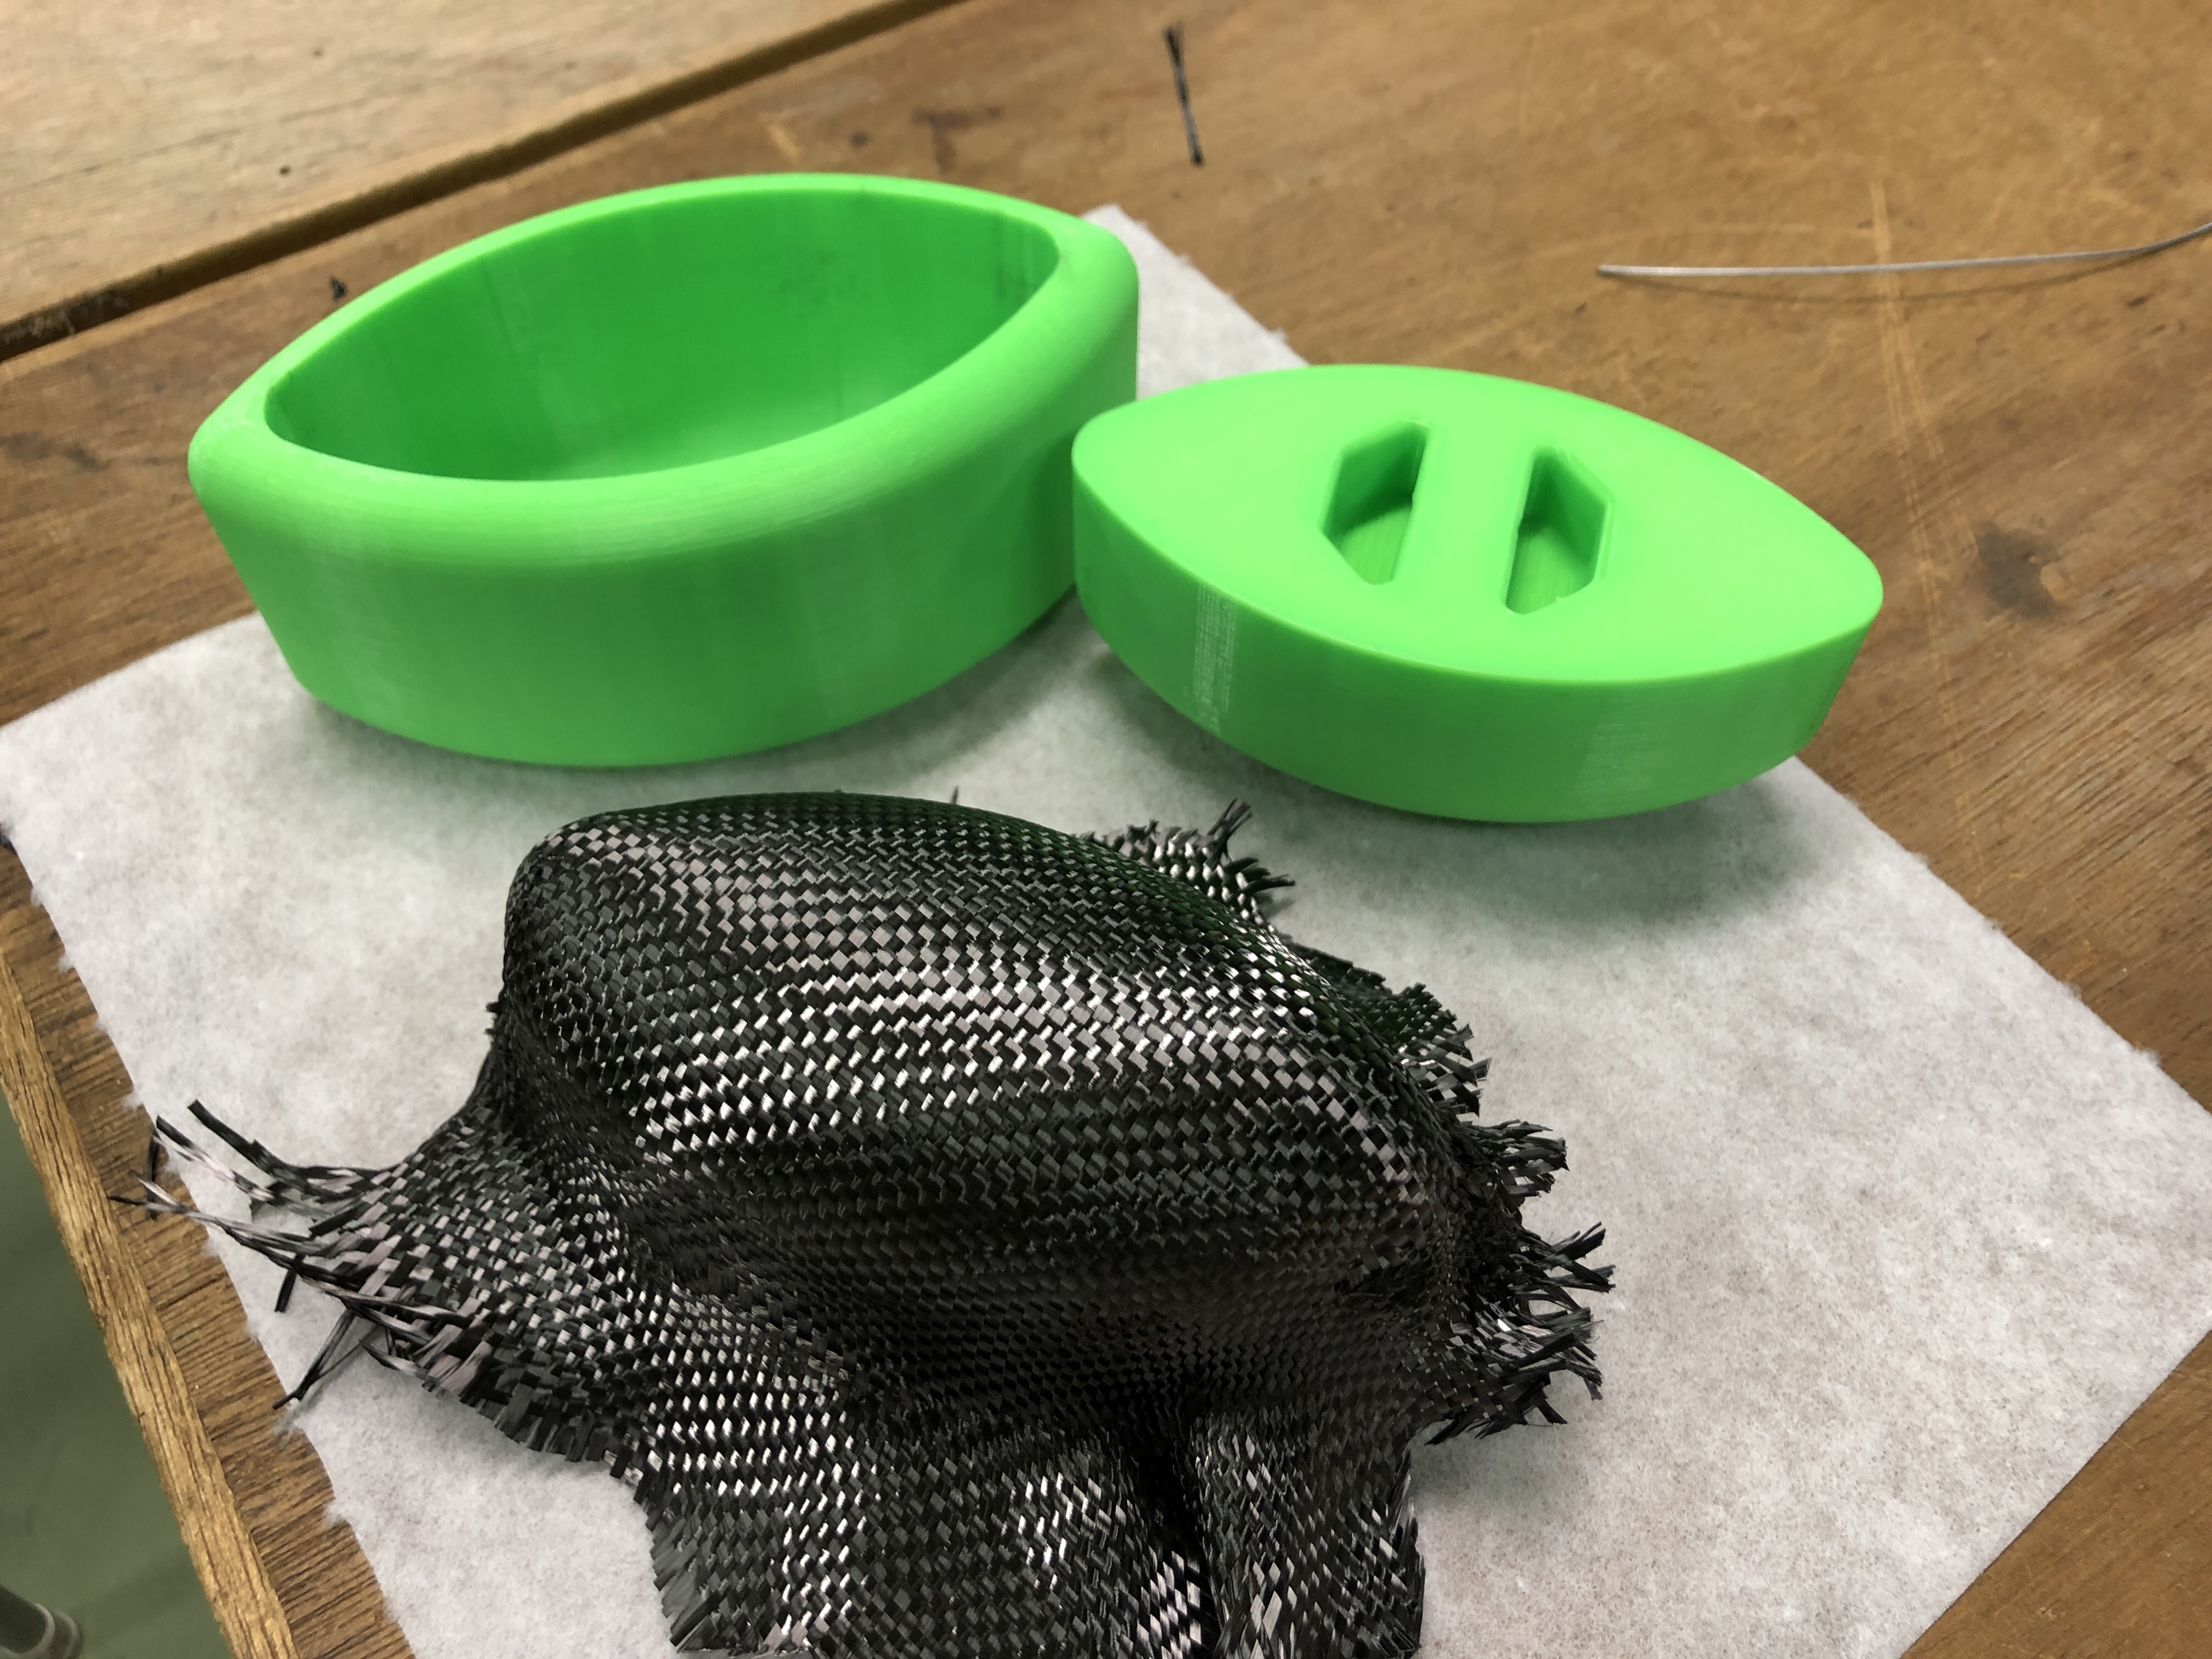
\includegraphics[width=120mm]{img/27.JPG}
    \end{center}
  \caption{雄型と雌型}
 \label{fig:robot}
\end{figure}

\begin{figure}[htbp]
  \begin{center}
    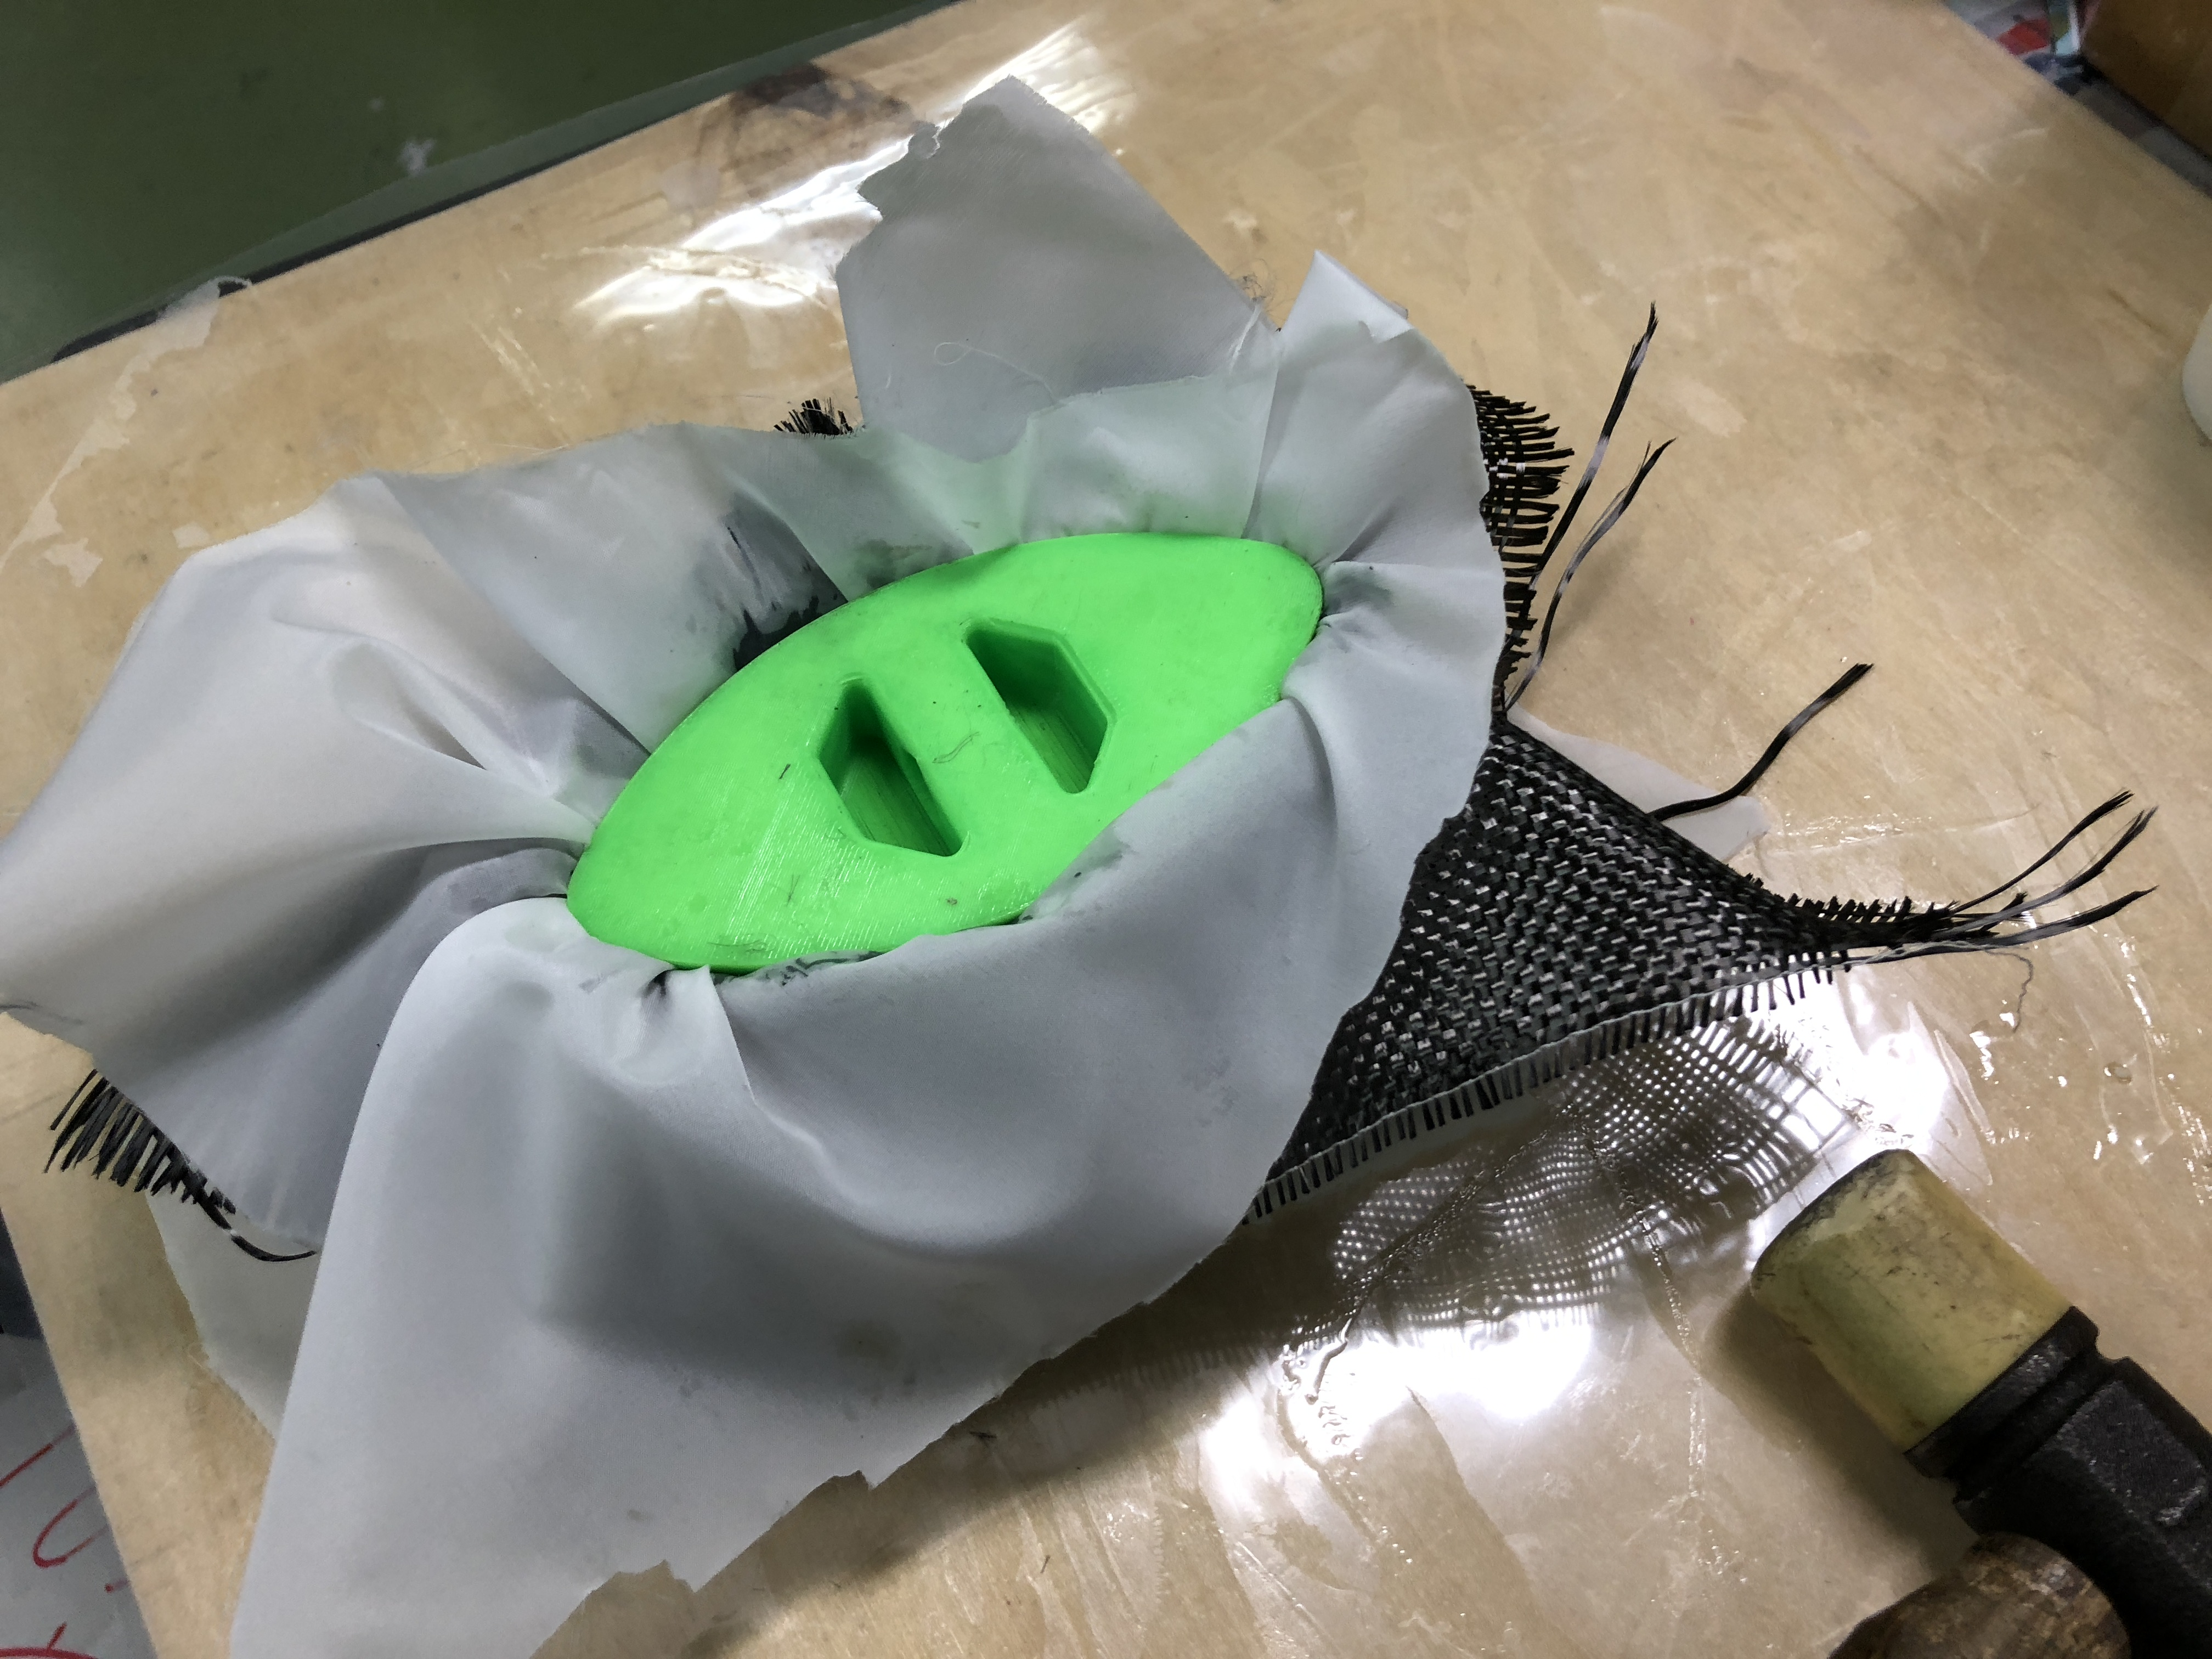
\includegraphics[width=120mm]{img/28.JPG}
    \end{center}
  \caption{はめ合わせ後の型}
 \label{fig:robot}
\end{figure}


